% \documentclass[11pt,twoside]{book} %纸质版用twoside
\documentclass[12pt,oneside]{book} %电子版用oneside
\usepackage{setspace}

% \documentclass{article}

%%%%%%%%%%%%%%%%%%%%%%%%%%%%%%%%%%%%%%%%%%%%%%%%%%
%%%%%%%%%%%%%%%%%%%%% preamble %%%%%%%%%%%%%%%%%%%
%%%%%%%%%%%%%%%%%%%%%%%%%%%%%%%%%%%%%%%%%%%%%%%%%%

\usepackage[mono=false]{libertine} % new linux font, ignore mono

\usepackage{luatex85}

%\renewcommand{\baselinestretch}{1.05}
\usepackage{amsmath,amsthm,amssymb,mathrsfs,amsfonts,dsfont}
\usepackage{epsfig,graphicx}
\usepackage{tabularx}
\usepackage{blkarray}
\usepackage{slashed}
\usepackage{color}
\usepackage{listings}
\usepackage{caption}
% \usepackage{fullpage}
\usepackage{lipsum} % provides dummy text for testing
\usepackage[toc,title,titletoc,header]{appendix}
\usepackage{minitoc}
\usepackage{color}
\usepackage{multicol} % two-col ToC
\usepackage{bm}
\usepackage{imakeidx} % before hyperref
\usepackage{hyperref}
\usepackage{indentfirst}
\setlength{\parindent}{2em}


% link colors settings
\hypersetup{
    colorlinks=true,
    citecolor=magenta,
    linkcolor=blue,
    filecolor=green,      
    urlcolor=cyan,
    % hypertexnames=false,
}
\usepackage[capitalise]{cleveref}
\usepackage{subcaption}
\usepackage{enumitem}
\usepackage{mathtools}
\usepackage{physics}
\usepackage[linesnumbered,ruled,vlined,algosection]{algorithm2e}
\SetCommentSty{textsf}
\usepackage{epigraph}
\epigraphwidth=1.0\linewidth
\epigraphrule=0pt

% adjust margin
\usepackage[margin=2.3cm]{geometry}
\headheight13.6pt


\usepackage{graphicx}
\usepackage[justification=centering]{caption} % 图注居中
\usepackage{setspace}
\usepackage{geometry}
\usepackage{float}
\usepackage{hyperref}
\usepackage[utf8]{inputenc}
\usepackage[english]{babel}
\usepackage{framed}


\newcommand{\HRule}[1]{\rule{\linewidth}{#1}}





\setstretch{1.2}
% \geometry{
%     textheight=9in,
%     textwidth=5.5in,
%     top=1in,
%     headheight=12pt,
%     headsep=25pt,
%     footskip=30pt
% }





%%%%%%%%%%%%%%%% thmtools %%%%%%%%%%%%%%%%%%%%%

\usepackage{thmtools}
\usepackage[dvipsnames]{xcolor}
\usepackage[most]{tcolorbox}
\usepackage{enumerate}

\colorlet{LightGreen}{Green!15} %def
\colorlet{LightBlue}{Blue!15} %thm
\colorlet{LightOrange}{Orange!15} %lem
\colorlet{LightGray}{Gray!15}  %prop
\colorlet{LightRed}{Red!40} %cor
\colorlet{LightYellow}{Yellow!15} %exa


% \newtcbtheorem[
%   number within = chapter % 按每个 chapter 分别编号
% ]{definition% 环境名
% }{Definition% 这个参数可以设成“定理”“引理”“推论”等,编号就会变成“定理 1.1”“引理 1.1”“推论 1.1”等
% }{
%   attach title to upper = \par\vspace{1ex}, % 不要单独的标题栏,定理名完了之后分段,加上适量空白
%   separator sign = \quad, % 定理编号和定理名字之间用什么分隔;默认是冒号
%   sharp corners, % 直角;默认是圆角
%   enhanced jigsaw, frame hidden, % 隐藏 tcb 边框
%   colback = LightGreen, % 背景色
%   coltitle = blue!20!cyan!80!black, % 标题(定理编号和名字)的颜色
%   fonttitle = \sffamily\small, % 标题(定理编号和名字)的字体
%   description font = \normalsize, % 定理名字的字体
%   fontupper = \normalfont, % box 内的字体
% }{def% label 前缀
% }

\newtcbtheorem[
  auto counter,number within = chapter % 按每个 chapter 分别编号
]{definition% 环境名
}{Definition% 这个参数可以设成“定理”“引理”“推论”等,编号就会变成“定理 1.1”“引理 1.1”“推论 1.1”等
}{
  sharp corners, % 直角;默认是圆角
  colback=Green!5,
  colframe=Green!50!black,
  fonttitle=\sffamily\small
}{def% label 前缀
}


% 计数器设置
\makeatletter
\renewcommand\theHtcb@cnt@definition{\thechapter.\arabic{tcb@cnt@definition}}
\makeatother

\newtcbtheorem[
  auto counter,number within = chapter % 按每个 chapter 分别编号
]{theorem% 环境名
}{Theorem% 这个参数可以设成“定理”“引理”“推论”等,编号就会变成“定理 1.1”“引理 1.1”“推论 1.1”等
}{
  sharp corners, % 直角;默认是圆角
  colback=yellow!10,
  colframe=yellow!50!black,
  fonttitle=\sffamily\small
}{thm% label 前缀
}
% 计数器设置
\makeatletter
\renewcommand\theHtcb@cnt@theorem{\thechapter.\arabic{tcb@cnt@theorem}}
\makeatother

\newtcbtheorem[
  auto counter,number within = chapter % 按每个 chapter 分别编号
]{proposition% 环境名
}{Proposition% 这个参数可以设成“定理”“引理”“推论”等,编号就会变成“定理 1.1”“引理 1.1”“推论 1.1”等
}{
  sharp corners, % 直角;默认是圆角
  colback=Red!5,
  colframe=Red!50!black,
  fonttitle=\sffamily\small
}{prop% label 前缀
}
% 计数器设置
\makeatletter
\renewcommand\theHtcb@cnt@proposition{\thechapter.\arabic{tcb@cnt@proposition}}
\makeatother

\newtcbtheorem[
  auto counter,number within = chapter % 按每个 chapter 分别编号
]{corollary% 环境名
}{Corollary% 这个参数可以设成“定理”“引理”“推论”等,编号就会变成“定理 1.1”“引理 1.1”“推论 1.1”等
}{
  sharp corners, % 直角;默认是圆角
  colback=Blue!5,
  colframe=Blue!50!black,
  fonttitle=\sffamily\small
}{cor% label 前缀
}

% 计数器设置
\makeatletter
\renewcommand\theHtcb@cnt@corollary{\thechapter.\arabic{tcb@cnt@corollary}}
\makeatother

\newtcbtheorem[
  auto counter,number within = chapter % 按每个 chapter 分别编号
]{lemma% 环境名
}{Lemma% 这个参数可以设成“定理”“引理”“推论”等,编号就会变成“定理 1.1”“引理 1.1”“推论 1.1”等
}{
  sharp corners, % 直角;默认是圆角
  colback=Gray!10,
  colframe=Gray!50!black,
  fonttitle=\sffamily\small
}{lem% label 前缀
}

% 计数器设置
\makeatletter
\renewcommand\theHtcb@cnt@lemma{\thechapter.\arabic{tcb@cnt@lemma}}
\makeatother


\newtcbtheorem[
  auto counter,number within = chapter % 按每个 chapter 分别编号
]{example}
{Example}%
  {
    enhanced, breakable,
    colback = white, colframe = purple, colbacktitle = purple,
    attach boxed title to top left = {yshift = -2mm, xshift = 5mm},
    boxed title style = {sharp corners},
    fonttitle=\sffamily\small
  }
{exa}

% 计数器设置
\makeatletter
\renewcommand\theHtcb@cnt@example{\thechapter.\arabic{tcb@cnt@example}}
\makeatother


\newtcbtheorem[
  auto counter,number within = chapter % 按每个 chapter 分别编号
]{exercise}
{Exercise}%
  {
    enhanced, breakable,
    colback = white, colframe = cyan, colbacktitle = cyan,
    attach boxed title to top left = {yshift = -2mm, xshift = 5mm},
    boxed title style = {sharp corners},
    fonttitle=\sffamily\small
  }
{exer}

% 计数器设置
\makeatletter
\renewcommand\theHtcb@cnt@exercise{\thechapter.\arabic{tcb@cnt@exercise}}
\makeatother


% \declaretheorem[numberwithin=chapter,shaded={rulecolor=LightGreen,
% rulewidth=2pt,bgcolor=LightGreen,
% textwidth=12em}]{definition}

\usepackage{changepage}
\newenvironment{remark}{\underline{\textbf{Remark.}}}{\par}

\newenvironment{proofsolution}
    {\renewcommand\qedsymbol{$\square$}\color{blue}\begin{adjustwidth}{0em}{2em}\begin{proof}[\textit Proof.~]}
    {\end{proof}\end{adjustwidth}}


%%%%%%%%%%%%%%%% index %%%%%%%%%%%%%%%%%%%%%
\begin{filecontents}{index.ist}
% https://tex.stackexchange.com/questions/65247/index-with-an-initial-letter-of-the-group
headings_flag 1
heading_prefix "{\\centering\\large \\textbf{"
heading_suffix "}}\\nopagebreak\n"
delim_0 "\\nobreak\\dotfill"
\end{filecontents}
\newcommand{\myindex}[1]{\index{#1} \emph{#1}}
\makeindex[columns=3, intoc, title=Alphabetical Index, options= -s index.ist]
%%%%%%%%%%%%%%%% index %%%%%%%%%%%%%%%%%%%%%

%%%%%%%%%%%%%%%% ToC %%%%%%%%%%%%%%%%%%%%%
% Link Chapter title to ToC: https://tex.stackexchange.com/questions/32495/linking-the-section-text-to-the-toc
\usepackage[explicit]{titlesec}
\titleformat{\chapter}[display]
  {\normalfont\huge\bfseries}{\chaptertitlename\ {\thechapter}}{20pt}{\hyperlink{chap-\thechapter}{\Huge#1}
\addtocontents{toc}{\protect\hypertarget{chap-\thechapter}{}}}
\titleformat{name=\chapter,numberless}
  {\normalfont\huge\bfseries}{}{-20pt}{\Huge#1}

%%%%%%%%%%%%%%%%%%% fancyhdr %%%%%%%%%%%%%%%%%
\usepackage{fancyhdr}
\pagestyle{fancy} % enable fancy page style
\renewcommand{\headrulewidth}{0.0pt} % comment if you want the rule
\fancyhf{} % clear header and footer
\fancyhead[lo,le]{\leftmark}
\fancyhead[re,ro]{\rightmark}
\fancyfoot[CE,CO]{\hyperref[toc-contents]{\thepage}}

% https://tex.stackexchange.com/questions/550520/making-each-page-number-link-back-to-beginning-of-chapter-or-section
\makeatletter
\def\chaptermark#1{\markboth{\protect\hyper@linkstart{link}{\@currentHref}{Chapter \thechapter ~ #1}\protect\hyper@linkend}{}}
\def\sectionmark#1{\markright{\protect\hyper@linkstart{link}{\@currentHref}{\thesection ~ #1}\protect\hyper@linkend}}
\makeatother
%%%%%%%%%%%%%%%%%%% fancyhdr %%%%%%%%%%%%%%%%%


%%%%%%%%%%%%%%%%%%% biblatex %%%%%%%%%%%%%%%%%
\usepackage[doi=false,url=false,isbn=false,style=alphabetic,backend=biber,backref=true]{biblatex}
\addbibresource{bib.bib}

\newbibmacro{string+doiurlisbn}[1]{%
  \iffieldundef{doi}{%
    \iffieldundef{url}{%
      \iffieldundef{isbn}{%
        \iffieldundef{issn}{%
          #1%
        }{%
          \href{http://books.google.com/books?vid=ISSN\thefield{issn}}{#1}%
        }%
      }{%
        \href{http://books.google.com/books?vid=ISBN\thefield{isbn}}{#1}%
      }%
    }{%
      \href{\thefield{url}}{#1}%
    }%
  }{%
    \href{http://dx.doi.org/\thefield{doi}}{#1}%
  }%
}

% https://tex.stackexchange.com/questions/94089/remove-quotes-from-inbook-reference-title-with-biblatex
\DeclareFieldFormat[article,incollection,inproceedings,book,misc]{title}{\usebibmacro{string+doiurlisbn}{\mkbibemph{#1}}}
% https://tex.stackexchange.com/questions/454672/biblatex-journal-name-non-italic
\DeclareFieldFormat{journaltitle}{#1\isdot}
\DeclareFieldFormat{booktitle}{#1\isdot}
% https://tex.stackexchange.com/questions/10682/suppress-in-biblatex
\renewbibmacro{in:}{}
% add video field: https://tex.stackexchange.com/questions/111846/biblatex-2-custom-fields-only-one-is-working
\DeclareSourcemap{
    \maps[datatype=bibtex]{
      \map{
        \step[fieldsource=video]
        \step[fieldset=usera,origfieldval]
    }
  }
}
\DeclareFieldFormat{usera}{\href{#1}{\textsc{Online video}}}
\AtEveryBibitem{
    \csappto{blx@bbx@\thefield{entrytype}}{% put at end of entry
        \iffieldundef{usera}{}{\space \printfield{usera}}
    }
}


%%%%%%%%%%%%%%%%%%%%%%%notations%%%%%%%%%%%%%%%%%%%%%%%%%%%%%%
\newcommand{\F}{\ensuremath{\mathbb{F}}}
\newcommand{\C}{\ensuremath{\mathbb{C}}} 
\newcommand{\R}{\ensuremath{\mathbb{R}}}
\newcommand{\J}{\ensuremath{\mathbb{J}}}
\newcommand{\Q}{\ensuremath{\mathbb{Q}}}
\newcommand{\Z}{\ensuremath{\mathbb{Z}}}
\newcommand{\N}{\ensuremath{\mathbb{N}}}
\newcommand{\K}{\ensuremath{\mathbb{K}}}
\newcommand{\Zo}{\ensuremath{\mathbb{Z}_{\geqslant 0}}} % 非负整数集
\newcommand{\Zi}{\ensuremath{\mathbb{Z}_{\geqslant 1}}} % 正整数集
\newcommand{\id}{\mathrm{id}}
\newcommand{\im}{\mathrm{im}\,}                         % 映射的像
\newcommand{\leqs}{\leqslant}
\newcommand{\geqs}{\geqslant}
\newcommand{\ci}{\mathrm{i}}
\newcommand{\hH}{\mathscr{H}}
\newcommand{\hK}{\mathscr{K}}
\newcommand{\inner}[2]{\langle#1,#2\rangle}

%%%%%%%%%%%%%%%%%%% biblatex %%%%%%%%%%%%%%%%%

%%%%%%%%%%%%%%%%%%%%% glossaries %%%%%%%%%%%%%%%%%
% !TEX root = ./notes_template.tex
% \usepackage[style=super]{glossaries}
% https://www.overleaf.com/learn/latex/Glossaries
\usepackage[style=super,toc,acronym]{glossaries}
\setlength{\glsdescwidth}{1\linewidth}
\makeglossaries

\renewcommand\glossaryname{List of Abbreviations and Symbols}

\newglossaryentry{Q2}{name={$Q_2(f)$},
%sort=Q2,
description={Two-side (bounded) error quantum query complexity}}

\newglossaryentry{real_number}{name={$\mathbb{R}$},description={Real number}}

% \newglossaryentry{gcd}{name={gcd},description={greatest common divisor}}

\newacronym{gcd}{GCD}{Greatest Common Divisor}


\newglossaryentry{svm}{name={SVM},description={Support Vector Machine}}

\newglossaryentry{gd}{name={GD},description={Gradient Descent}}

\newglossaryentry{qft}{name={QFT},description={Quantum Field Theory}}

\newglossaryentry{qm}{name={QM},description={Quantum Mechanics}}

\newglossaryentry{v}{name={$\vec{v}$},description={a vector}}

% physics
\newglossaryentry{hamiltonian}{name={$\hat{H}$},description={Hamiltonian}}

\newglossaryentry{lagrangian}{name={$L$},description={Lagrangian}}
%%%%%%%%%%%%%%%%%%%%% glossaries %%%%%%%%%%%%%%%%%

%%%%%%%%%%%%%%%%%%%%% glossaries-extra %%%%%%%%%%%%%%%%%
% \usepackage[record,abbreviations,symbols,stylemods={list,tree,mcols}]{glossaries-extra}
%%%%%%%%%%%%%%%%%%%%% glossaries-extra %%%%%%%%%%%%%%%%%


% !TEX root = ./notes_template.tex

%%%%%%%%%%%%%%%%%%%%%%%%%%%%%%%%%%%%
%%%%%%%%%%%%%%%%%%%%%%%%%%%%%%%%%%%%
% math
\let\iff\relax
\newcommand{\iff}{\text{ iff }}
\newcommand{\OPT}{\textup{OPT}}

% physics
\newcommand{\acreation}{a^\dagger}



%%%%%%%%%%%%%%%%%%%%%%%%%%%%%%%%%%%%%%%%%%%%%%%%%%
%%%%%%%%%%%%%%%% begin of document %%%%%%%%%%%%%%%
%%%%%%%%%%%%%%%%%%%%%%%%%%%%%%%%%%%%%%%%%%%%%%%%%%

\begin{document}

\title{\bf \huge Study Notes of Abtract Algebra}
\author{Pei Zhong}
\date{Update on \today}

\maketitle

% \newpage
% \let\cleardoublepag\clearpage

\tableofcontents

\begin{spacing}{1}

%%%%%%%%%%%%%%update progress%%%%%%%%%%



%%%%%%%%%%%%%%update progress end%%%%%%%%




%%%%%%%%%%%%%%%preface%%%%%%%%%%%%%

\chapter*{Preface}

Notes mainly refer to following materials:


\begin{itemize}
    \item[*] Machine learning
    \begin{itemize}
        \item \href{https://www.cs.cornell.edu/courses/cs4780/2023sp/}{lecture notes from cornell}
        \item \href{https://www.cs.cmu.edu/~hn1/documents/machine-learning/notes.pdf}{lecture notes from cmu}
        \item \href{https://cs229.stanford.edu/main_notes.pdf}{lecture notes of CS229}
    \end{itemize}
    \item[*] Deep learning
    \begin{itemize}
        \item \href{https://udlbook.github.io/udlbook/}{understanding deep learning}
        \item \href{https://www.bilibili.com/video/BV1Wv411h7kN/?spm_id_from=333.337.search-card.all.click}{lecture video from Hongyi Lee}
        \item \href{https://cs231n.github.io/}{lecture notes from Stanford}
    \end{itemize}
    \item[*] Reinforcement learning
    \begin{itemize}
        \item \href{https://web.stanford.edu/class/cs234/modules.html}{lecture notes from stanford}
        \item \href{https://people.cs.umass.edu/~bsilva/courses/CMPSCI_687/Fall2022/Lecture_Notes_v1.0_687_F22.pdf}{lecture notes from umass}
    \end{itemize}
\end{itemize}







\chapter{Preliminary Knowledge}


%%%%%%%%%%%%%preface end%%%%%%%%%%%%%
\part{Group Theory}
\chapter{Semi-Group and Group}\label{chp:1_2}

\begin{definition}{}{}
    If $G$ is a nonempty set, 
    then a binary operation on $G$ is a function
    from $G \times G$ to $G$. 
    If the binary operation is denoted $\circ$, 
    then we use the notation
    $a \circ b = c$ 
    if $(a, b) \in G \times G$ is mapped to $c \in G$ 
    under the binary operation.
\end{definition}

\begin{remark}
    We will consider both "additive" and "multiplicative" binary operations.
    The only difference between these operations is notational, really. 
    When considering a binary operation, we denote the image of $(a, b)$ as $a + b$. 
    When using multiplicative notation, we denote the image of $(a, b)$ as $ab$ 
    (called the product of $a$ and $b$). 
    Throughout the group theory we use multiplicative notation.
\end{remark}

\begin{definition}{}{definition of group}
    For a multiplicative binary operation on $G\times G$,
    we define the following properties:\\
    (1) Multiplication is associative if $a(bc)=(ab)c$ for all $a,b,c\in G$.\\
    (2) Element $e\in G$ is a identity if $ae=ea=a$ for all $a\in G$.\\
    (3) Element $a\in G$ has a inversee $b$ 
    if for some $b\in G$ we have $ab=ba=e$.\\
    A semigroup is a nonempty set $G$ with an associative binary operation.\\
    A monoid is a semigroup with an identity.\\
    A group is a monoid such that each $a\in G$ has an inverse.\\
    In a semigroup, we define the property:\\
    (4) Semigroup $G$ is abelian or commutative if $ab=ba$ for all $a,b\in G$.\\
    The order of a semigroup/monoid/group is the cardinality of set $G$, denoted $|G|$.
    If $|G| < \infty$, then the semigroup/monoid/group is said to be finite.
\end{definition}

\begin{remark}
    If we define a binary algebraic structure as a set with a binary operation on
    it, then we have the following schematic:\\

    \hspace{2cm}(Binary Algebraic Structures) $\supseteq$ (Semigroups) $\supseteq$ (Monoids) $\supseteq$ (Groups).
\end{remark}

\begin{proposition}{Generalized Associative Law}{}
    Let $G$ be a semigroup. For any $a_1,...,a_n\in G$, 
    the value of $a_1\cdots a_n$
    is independent of how the expression is bracketed.
\end{proposition}

\begin{proposition}{Generalized Commutative Law}{Generalized Commutative Law}
    If $G$ is a commutative semigroup and $a_1, a_2, . . . , a_n \in G$ 
    then for any permutation
    $i_1, i_2, . . . , i_n$ of $i = 1, 2, . . . , n$
     we have the products $a_1a_2 \cdots a_n = a_{i_1} a_{i_2}\cdots a_{i_n}$.
\end{proposition}

\begin{definition}{}{}
    Let $G$ be a (multiplicative) semigroup, $a \in G$, and $n \in \N$. 
    The element $a^n$ is defined as 
    the standard $n$ product $a^n =\prod_{i=1}^{n}a_i$
    where $a = a_i$ for $1 \leqs i \leqs n$. 
    If $G$ is a monoid, $a^0$ is defined to be the identity element of $G$, 
    $a^0=e$. If $G$ is a group, 
    then for each $n \in \N$, $a^{-n}$
    is defined to be $a^{-n} = (a^{-1})^n\in G$.
    If $G$ is an additive group we replace $a^n, a^0, a^{-n}$, and $e$ 
    with $na, 0a, -na$, and $0$, respectively.
\end{definition}

\begin{proposition}{}{}
    If $G$ is a group (respectively, semigroup, monoid) and $a \in G$,
    then for all $m, n \in \Z$ (respectively, $\N$, $\N \cup \{0\}$):
    (1) $a^ma^n=a^{m+n}$ (or $ma + na = (m + n)a$ in additive notation);
    \\
    (2) $(a^m)^n=a^{mn}$(or $n(ma) = (mn)a$ in additive notation).
\end{proposition}

\begin{proposition}{}{}
    If G is a monoid, then the identity element $e$ is unique. If $G$ is a group then:\\
    (1) If $c \in G$ and $cc = c$ then $c = e$.\\
    (2) For all $a,b\in G$, if $ab=ac$ then $b=c$, 
    and if $ba=ca$ then $b=c$ (these properties
    of a group is called left cancellation and right cancellation, respectively).\\
    (3) For $a\in G$, the inverse of $a$ is unique.\\
    (4) For all $a\in G$, we have $(a^{-1})^{-1}=a$.\\
    (5) For all $a,b\in G$, we have $(ab)^{-1}=b^{-1}a^{-1}$.\\
    (6) For all $a,b\in G$, the equations $ax=b$ and $ya=b$ have unique solutions in $G$,
    namely $x=a^{-1}b$ and $y=ba^{-1}$, respectively.
\end{proposition}

\begin{remark}
    We can weaken the two-sided identity and inverse properties used in Definition \ref{def:definition of group} 
    of group. It turns out that if we simply assume right inverses and a right
    identity (or just left inverses and a left identity) then this implies the existence of
    left inverses and a left identity (and conversely), as shown in the following theorem.
\end{remark}

\begin{proposition}{}{}
    Let $G$ be a semigroup. 
    Then $G$ is a group if and only if the
    following conditions hold.\\
    (1) There exists an element $e \in G$ such that $ea = a$ for all $a \in G$ (called a left
    identity in G).
    (ii) For each $a \in G$, there exists an element $a^{-1}\in G$ such that $a^{-1}a=e$
    ($a^{-1}$ is called a left inverse of a).
\end{proposition}

The following proposition gives another condition by which a semigroup is
a group.

\begin{proposition}{}{}
    (1) Let $G$ be a semigroup. Then $G$ is a group if and only if for
    all $a, b \in G$ the equations $ax = b$ and $ya = b$ have solutions in $G$.\\
    (2) Let $G$ be a finite semigroup, if $G$ satisfys cancellation law, then $G$ is a group.
\end{proposition}

\section{Reference}

\begin{itemize}
    \item \href{https://faculty.etsu.edu/gardnerr/5410/notes/I-1.pdf}{Semigroups, Monoids, and Groups}
\end{itemize}
\chapter{Examples of Group}\label{chp:1_3}


\chapter{Subgroup and Coset}\label{chp:1_4}

\section{Subgroups}

\begin{definition}{}{}
    Let $G$ be a semigroup and $H$ a nonempty subset of $G$.
    If for every $a,b\in H$ we have $ab\in H$ then $H$ is closed under the binary operation of $G$.
    Let $G$ be a group and $H$ a nonempty subset of $G$ that is closed under the binary operation of $G$.
    If $H$ itself is a group under the binary operation then $H$ is a subgroup of $G$.
    This is denote $H\leqs G$. For group $G$, 
    the trivial subgroup is $\{e_G\}$.
    Subgroup $H\leqs G$ is a proper subgroup if $H\neq G$ and $H\neq \{e_G\}$.
\end{definition}

\begin{proposition}{}{}
    Let $H$ be a nonempty subset of a group $G$. 
    Then $H$ is a subgroup of $G$ 
    if and only if $ab^{-1} \in H$
    for all $a, b \in H$.
\end{proposition}

\begin{example}{}{}
    $\Q^*\leqs \R^*\leqs \C^*$
\end{example}

\begin{example}{}{}
    $\text{SL}_n(\R)\leqs \text{GL}_n(\R)$.
\end{example}

\begin{corollary}{}{}
    If $G$ is a group and $\{H_i:i\in I\}$ is a nonempty set of subgroup of $G$,
    then $\cap_{i\in I}H_i$ is a subgroup of $G$.
\end{corollary}
\begin{remark}
    Notice that index set $I$ may not be finite and
    it may not even be countable!
\end{remark}


\begin{definition}{}{}
    Let $G$ be a group and $X,Y\subseteq G$.
    $X^{-1}$ is defined as $X^{-1}=\{x^{-1}:x\in X\}$. 
    And $XY$ is defined as $XY=\{xy:x\in X\text{ and } y\in Y\}$.
\end{definition}

\begin{proposition}{}{}
    Let $G$ be a group and $X,Y,Z\subseteq G$, then
    $(X^{-1})^{-1}=X$ and $(XY)Z=X(YZ)$.
\end{proposition}

\begin{proposition}{}{}
    Let $G$ be a group and $H\leqs G$, then
    $H^{-1}=H$ and $HH=H$.
\end{proposition}

\begin{proposition}{}{}
    Let $G$ is a group and $H,K\leqs G$, then
    \begin{align*}
        HK\leqs G\Leftrightarrow HK=KH.
    \end{align*}
\end{proposition}

\section{Cosets}
In this section, we generalize the idea of congruence modulo $m$ on $\Z$ (Chapter\ref{chp:pre1}) to 
a more general setting.

\begin{definition}{}{}
    Let $H$ be a subgroup of group $G$ and $a,b\in G$.
    $a$ is right congruent to $b$ modulo $H$, denoted $a\equiv_r b\pmod H$, if $ab^{-1}\in H$.
    $a$ is left congruent to $b$ modulo $H$, denoted by $a\equiv_l b\pmod H$, if $a^{-1}b\in H$.
\end{definition}

We use left and right congruent to define left and right cosets. 

\begin{theorem}{}{}
    Let $H$ be a subgroup of a group $G$.\\
    (1) Right and left congruence modulo $H$ are each equivalence relations on $G$.\\
    (2) The equivalence class of $a\in G$ under right (and left) congruence modulo $H$ is 
    the set $Ha=\{ha:h\in H\}$ (and $aH={ah:h\in H}$ for left congruence).\\
    (3) $|Ha|=|H|=|aH|$ for all $a\in G$. \\
    The set $Ha$ is a right coset of $H$ in $G$ and $aH$ is a left coset of $H$ in $G$.
\end{theorem}

\begin{corollary}{}{}
    Let $H$ be a subgroup of group $G$.\\
    (1) $G$ is the union of the right (and left) cosets of $H$ in $G$.\\
    (2) Two right (or two left) cosets of $H$ in $G$ are either disjoint or equal.\\
    (3) For $a,b\in G$, we have $Ha=Hb$ if and only if $ab^{-1}\in H$, and $aH=bH$ if and only if $a^{-1}b\in H$.\\
    (4) If $\mathcal{R}$ is the set of distinct right cosets of $H$ in $G$ and $\mathcal{L}$ is the set of distinct left cosets of $H$ in $G$,
    then $|\mathcal{R}|=|\mathcal{L}|$.
\end{corollary}
\begin{remark}
    (1)(2) imply that the right (and left) cosets of $H$ in $G$ partition $G$.
\end{remark}

\begin{definition}{}{}
    Let $H$ be a subgroup of a group $G$.
    The index of $H$ in $G$,
    denoted $[G : H]$, 
    is the cardinal number of the set of distinct right (or left) cosets
    of $H$ in $G$.
\end{definition}

\begin{theorem}{}{}
    Let $G$ be a finite group and $H\leqs G$,
    then $|H|$ divides $|G|$ and $|G|=[G:H]|H|$.
\end{theorem}

\begin{remark}{}{}
    The converse of the Lagrange's Theorem does
    not hold. For example, the alternating group $A_4$ of order 12 
    does not have a subgroup of order $6$. So
    it is natural to ask: "For a given divisor $d$ 
    of the order of a finite group $G$, under
    what conditions does $G$ have a subgroup of order $d$?" 
    This is partially addressed by The Sylow Theorems (see chapter\ref{chp:2_3}).
\end{remark}


\section{Reference}
\begin{itemize}
    \item \href{https://faculty.etsu.edu/gardnerr/5410/notes/I-2.pdf}{Subgroup}
    \item \href{https://faculty.etsu.edu/gardnerr/5410/notes/I-4.pdf}{Cosets}
\end{itemize}
\chapter{Normal Subgroup and Qutient Subgroup}\label{chp:1_7}

\begin{proposition}{}{normal equivalent}
    If $N$ is a subgroup of group $G$, then the following conditions are equivalent.\\
    (1) $aN=Na$ for all $a\in G$.\\
    (2) For all $a\in G$, $n\in N$, $ana^{-1}\in N$.\\
    (3) For all $a\in G$, $aNa^{-1}=N$.
\end{proposition}

\begin{definition}{}{}
    A subgroup $N$ of a group $G$ 
    which satisfies the equivalent
    conditions of proposition \ref{prop:normal equivalent} 
    is said to be normal in $G$ (or a normal subgroup of $G$),
    denoted $N\unlhd G$.
\end{definition}

\begin{proposition}{}{}
    Every subgroup of an abelian group is normal.
\end{proposition}

\begin{proposition}{}{}
    Any subgroup $N$ of index 2 in group $G$ is a normal subgroup.
\end{proposition}

\begin{proposition}{}{}
    The intersection of any collection of normal subgroups
    of group $G$ is itself a normal subgroup.
\end{proposition}

\begin{proposition}{}{}
    Let $G$ be a group and $H\leqs K\leqs M$.
    If $H\unlhd G$, then $H\unlhd K$.
\end{proposition}

\begin{remark}
    It may be the case that for group $G$, 
    we have subgroups of $G$ satisfying
    $H\unlhd K$ and $K\unlhd G$ but $H$ 
    is not a normal subgroup of $G$.
\end{remark}

The following result is a big one! 
It says that if $N$ is a normal subgroup of
$G$, then we can form a group out of the cosets of $N$ 
by defining a binary operation on the cosets using representatives of the cosets. 
In fact, this can be done only
when $N$ is a normal subgroup, 
the group of cosets is called a "factor group" or "quotient group." 
Quotient groups are at the backbone of modern algebra!

\begin{theorem}{}{quotient group well defined}
    If $N$ is a normal subgroup of a group $G$ and $G/N$ is the set of 
    all left cosets of $N$ in $G$, 
    then $G/N$ is a group of order $[G:N]$ 
    under the binary operation given by $(aN)(bN)=(ab)N$.
\end{theorem}

\begin{remark}{}{}
    By the definition of the binary operation in $G/N$,
    we see that the identity element is $eN=N$,
    and the inverse of $aN$ is $a^{-1}N$.
\end{remark}

\begin{definition}{}{}
    If $N$ is a normal subgroup of $G$, then the group $G/N$
    of theorem\ref{thm:quotient group well defined}
    is the quotient group of $G$ by $N$.
\end{definition}
\begin{remark}
    The relationship between quotient groups 
    and normal subgroups is a little
    deeper than Theorem \ref{thm:quotient group well defined} 
    implies. From Fraleigh, we have:
    Let $H$ be a subgroup of a group $G$. 
    Then left coset multiplication is well defined by 
    $(aH)(bH) = (ab)H$ 
    if and only if H is a normal subgroup of $G$.
    This result gives the real importance of normal subgroups.
\end{remark}

\section{Reference}

\begin{itemize}
    \item \href{https://faculty.etsu.edu/gardnerr/5410/notes/I-5.pdf}{Normality, Quotient Groups}
\end{itemize}

\chapter{Group Homomorphism and Isomorphism}\label{chp:1_8}

\begin{definition}{}{}
    Let $G$ and $H$ be semigroups.
    A function $f:G\rightarrow H$ is a homomorphism
    if $f(ab)=f(a)f(b)$ for all $a,b\in G$.
    A one to one (injective) homomorphism is a monomorphism.
    An onto (surjective) homomorphism is an epimorphism.
    A one to one and onto (bijective) homomorphism is an isomorphism.
    If there is an isomorphism from $G$ to $H$, we say that
    $G$ and $H$ are isomorphic, denoted $G\cong H$. 
    A homomorphism $f:G\rightarrow G$ is an endomorphism of $G$.
    An isomorphism $f:G\rightarrow G$ is an automorphism of $G$. 
\end{definition}

\begin{proposition}{}{}
    If $f : G \rightarrow H$ and 
    $g : H \rightarrow K$ 
    are homomorphisms on semigroups $G, H, K$,
    then the composition $g \circ f = gf : G \rightarrow K$ 
    is a homomorphism. 
    Similarly, compositions of monomorphisms, epimorphisms, isomorphisms, and automorphisms are
    respectively monomorphisms, epimorphisms, isomorphisms, and automorphisms.
\end{proposition}

\begin{proposition}{}{}
    a group homomorphism maps identities to identities and inverses to inverses.
\end{proposition}

\begin{definition}{}{}
    Let $f:G\rightarrow H$ be a homomorphism of groups.
    The kernel of $f$ is $\text{Ker}(f)=\{g\in G:f(g)=e_H\in H\}$.
    If $A\subset G$, then the image of $A$ is $f(A)=\{h\in H:h=f(a) \text{ for some }a\in A\}$.
    The set $f(G)$ is called the image of homomorphism $f$, denoted $\text{Im}(f)$.
\end{definition}

\begin{proposition}{}{}
    Let $f:G\rightarrow H$ be a homomorphism of groups. Then:\\
    (1) $f$ is a monomorphism if and only if $\text{Ker}(f)=\{e_G\}$;\\
    (2) $f$ is an isomorphism if and only if there is a homomorphism
    $f^{-1}:H\rightarrow G$ such that $ff^{-1}=1_H$ and $f^{-1}f=1_G$.
\end{proposition}


\begin{theorem}{}{canonical epimorphism thm}
    If $f:G\rightarrow H$ is a homomorphism of groups,
    then the kernel of $f$ is a normal subgroup of $G$. Conversely,
    if $N$ is a normal subgroup of $G$,
    then the map $\pi: G\rightarrow G/N$ given by $\pi(a)=aN$ is an epimorphism
    (that is, an onto homomorphism) with kernel $N$.
\end{theorem}

\begin{definition}{}{}
    The map $\pi:G\rightarrow G/N$ of theorem \ref{thm:canonical epimorphism thm}
    defined as $\pi(a)=aN$ is the canonical epimorphism.
\end{definition}

\begin{theorem}{}{}
    If $f : G \rightarrow H$ 
    is a homomorphism of groups, 
    then $f$ induces an isomorphism of
    $G/\text{Ker}(f)$ with $\text{Im}(f)$. 
\end{theorem}

\begin{figure}[H]
    \centering
    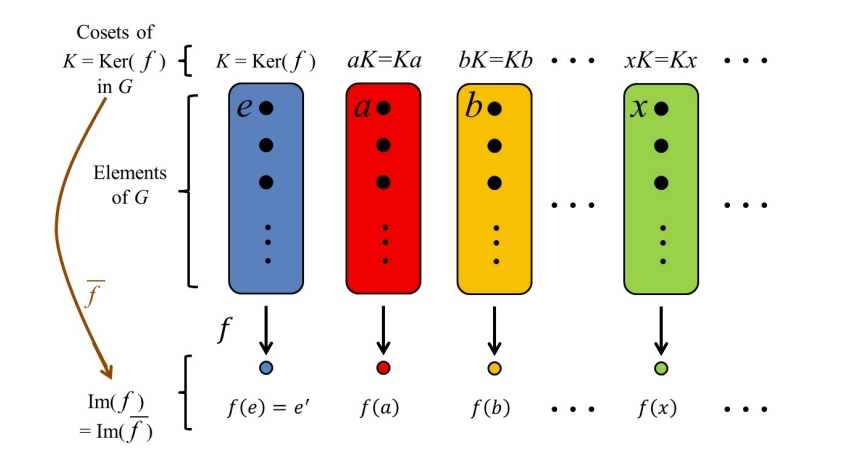
\includegraphics[width=0.6\textwidth]{figure/isomorphism.png}
    \caption{}
\end{figure}

\section{Reference}

\begin{itemize}
    \item \href{https://faculty.etsu.edu/gardnerr/5410/notes/I-2.pdf}{Homomorphisms}
    \item \href{https://faculty.etsu.edu/gardnerr/5410/notes/I-5.pdf}{Homomorphisms}
\end{itemize}



\chapter{Properties and Application of Index}\label{chp:1_5}

\begin{proposition}{}{}
    If $K, H, G$ are groups with $K \leqs H \leqs G$ and $[G:H],[H:K]$ are finite,
    then $[G : K] = [G :H][H : K]$. 
\end{proposition}

\chapter{Order of Element and Cyclic Group}\label{chp:1_6}

\section{Order of element and cyclic group}

\begin{definition}{}{}
    Let $G$ be a group and $X$ a subset of $G$.
    Let $\{H_i:i\in I\}$ be the set of all subgroups of $G$
    which contain $X$. Then $\cap_{i\in I}H_i$ is the subgroup of $G$
    generated by the set $X$, denoted $\geg{X}$.
\end{definition}

\begin{definition}{}{}
    For group $G$. the elements of $X\subset G$
    are called generators of subgroup $\geg{X}$.
    If $G=\geg{a_1,a_2,...,a_n}$ (notice the set brackets are dropped by convention)
    then $G$ is finitely generated.
\end{definition}

\begin{theorem}{}{}
    If $G$ is group and $X$ is a nonempty subset of $G$,
    then
    \begin{align*}
        \geg{X}=\{x_1^{m_1}x_2^{m_2}\cdots x_k^{m_k}:k\in \N_+, x_1,...,x_k\in X \text{ and } m_1,...,m_k\in\Z\}.
    \end{align*}
    In particular, for every $a\in G$, $\geg{a}=\{a^m:m\in\Z\}$.
\end{theorem}

\begin{definition}{}{}
    Let $G$ be a group. Then 
    $G$ is cyclic if $\exists a\in G$
    such that $G=\geg{a}=\{a^m:m\in\Z\}$.
\end{definition}

\begin{definition}{}{}
    Let $G$ be a group and $a\in G$.
    The order of $a$ is the least positive integer such that $a^n=e$,
    denoted $o(a)$. If such positive integer does not exist, $o(a)=\infty$.
\end{definition}

\begin{proposition}{}{}
    $o(a)=|\geg{a}|.$
\end{proposition}


We now explore the properties of elements of finite and infinite order.

\begin{proposition}{}{}
    Let $G$ be a group and $a\in G$.
    If $a$ has infinite order then\\
    (1) $a^k=e$ if and only if $k=0$.\\
    (2) the elements $a^k$ are all distinct as the values of $k$ range over $\Z$.\\
    If $a$ has finite order $m>0$ then \\
    (3) $a^k=e$ if and only if $m|k$.\\
    (4) $a^r=a^s$ if and only if $r\equiv s\pmod m$.\\
    (5) $\geg{a}$ consists of the distinct elements $a,a^2,...,a^{m-1},a^m=e$.\\
    (6) for each $k\in \Z$, $o(a^k)=\frac{m}{(m,k)}$, where $(m,k)=\text{gcd}(m,k)$. 
\end{proposition}

\begin{proposition}{}{}
    Let $G=\geg{a}$ be a cyclic group.
    If $G$ is infinite, then $a$ and $a^{-1}$ are the only generators of $G$.
    If $G$ is finite of order $m$, then $a^k$ is a generator of $G$ if and only if $(k,m)=1$ (i.e. $k$ and $m$ are coprime). 
\end{proposition}

\begin{proposition}{}{}
    The subgroup of cyclic group is cyclic.
\end{proposition}

\begin{proposition}{}{}
    Subgroup of infinite cyclic group is infinite cyclic group.
\end{proposition}


\begin{proposition}{}{}
    A finite cyclic group of order $n$ contains a subgroup of order m for each positive integer m which
divides n.
\end{proposition}

\begin{proposition}{}{}
    Every infinite cyclic group is isomorphic to the additive group $\Z$
    and every finite cyclic group of order $m$ 
    is isomorphic to the additive group $\Z_m$.
\end{proposition}

\begin{proposition}{}{}
    If a group $G$ has order $p^n$ where $p$
    is a prime, then $G$
    has a element of order $p$.
\end{proposition}

\begin{corollary}{}{}
    A group of order $p$ where $p$ is a prime number is cyclic.
\end{corollary}

\section{Application}
\begin{proposition}{}{}
    Let $G$ be a group of order $n$, then for $a\in G$, $a^n=e$.
\end{proposition}

\begin{definition}{}{}
    Euler's totient function counts the positive integers up to a given integer $n$ that are relatively prime to $n$. 
    It is written using $\varphi(n)$. 
\end{definition}

\begin{proposition}{}{}
    For $m\in \N_+$, $U_m:=\{\bar{a}=a+m\Z: a\in \Z \text{ and } \text{gcd}(a,m)=1\}$,
    then $U_m$ is a commutative semigroup with respect to multiplication 
    and $|U_m|=\varphi(m)$. If $U_m$ is finite, then $U_m$ is a abelian group.
\end{proposition}

\begin{theorem}{}{}
    If $m$ is a positive integer and $a$ is an integer such that $(a,m)=1$, then
    \begin{align*}
        a^{\varphi(m)}\equiv 1\pmod m.
    \end{align*}
\end{theorem}

\section{Reference}
\begin{itemize}
    \item \href{https://sites.millersville.edu/bikenaga/abstract-algebra-1/cyclic-groups/cyclic-groups.pdf}{cyclic group}
    \item \href{https://faculty.etsu.edu/gardnerr/5410/notes/I-3.pdf}{cyclic group}
\end{itemize}

\chapter{Group Action}\label{chp:2_1}



\begin{definition}{}{}
    An action of a group $G$ on a set $S$ is a function mapping $G\times S\rightarrow S$
    (denoted $(g,x)\mapsto g\circ x$) such that for all $x\in S$ and $g_1,g_2\in G$,
    we have
    \begin{align*}
        e\circ x=x\text{ and } (g_1g_2)\circ x=g_1\circ(g_2\circ x).
    \end{align*}
    When this occurs, we say that $G$ acts on set $S$.
\end{definition}






\begin{itemize}
    \item \href{https://faculty.etsu.edu/gardnerr/5410/notes/II-4.pdf}{Group Action}
\end{itemize}
\chapter{Sylow Theorem}\label{chp:2_3}

\begin{theorem}{Cauchy Theorem}{}
    If $G$ is a finite group whose order is divisible by a prime $p$, 
    then $G$ contains an element of order $p$.
\end{theorem}



\chapter{The Direct Product of Group}\label{chp:3_5}

\begin{definition}{}{}
  Let $(G,\circ)$ and $(H,\diamond)$ be groups. Put 
  \begin{align*}
    G\times H=\{(g,h):g\in G,h\in H\}
  \end{align*}
  with the operation  $(g_1,h_1)\times (g_2,h_2)=(g_1\circ g_2, h_1\diamond h_2)$. 
  Then $G\times H$ is a group, with identity $(1_G,1_H)$ and $(g,h)^{-1}=(g^{-1},h^{-1})$.
  It is called the outer direct product of $G$ and $H$.
\end{definition}
Similarly, there is a general case.
\begin{definition}{}{}
    Let $G_1,...,G_n$ be groups. Put 
    \begin{align*}
      G = G_1\times ...\times G_n=\{(x_1,...,x_n):x_i\in G_i\}
    \end{align*}
    with the operation  $(x_1,...,x_n)\times (y_1,...,y_n)=(x_1y_1,..., x_ny_n)$. 
    Then $G$ is a group, with identity $e = (e_1,...,e_n)$ and $(x_1,...,x_n)^{-1}=(x_1^{-1},...,x_n^{-1})$.
    It is called the outer direct product of $G_1,...,G_n$.
\end{definition}

Let's review the product of subgroups: 
\begin{proposition}{}{}
    Let $(G,\cdot)$ be a group and $X,Y\leqs G$, then
\begin{align*}
    XY = {x\cdot y:x\in X,y\in Y}.
\end{align*}
If $X<Y\unlhd G$, then $XY$ is a normal subgroup of $G$.
\end{proposition}




\begin{theorem}{}{}
    Put
    \begin{align*}
        G^* &= \{(g,1_H):g\in G\}.
        H^* &= \{(1_G,h):h\in H\}
    \end{align*}
    and define $\sigma_1 : G\times H\rightarrow H$ by $\sigma_1(g,h)=h$. Then\\
    (1) $\sigma_1$ is a homomorphism, $\Im \sigma_1 = H$ and $\Ker\sigma_1 = G^*$\\
    (2) $G^*\unlhd G\times H$ and $(G\times H)/G^*\cong H$.\\
    Similarly, define $\sigma_2 : G\times H\rightarrow G$ by $\sigma_2(g,h)=g$. Then\\
    (3) $\sigma_2$ is a homomorphism, $\Im \sigma_2 = G$ and $\Ker\sigma_2 = H^*$\\
    (4) $H^*\unlhd G\times H$ and $(G\times H)/H^*\cong G$.\\
    And more, \\
    (5) $G\cong G^*$ and $H\cong H^*$\\
    (6) $G^*H^*=G\times H$\\
    (7) $G^*\cap H^*=\{(1_G,1_H)\}$.
\end{theorem}

Similarly, there is general case.

\begin{theorem}{}{}
    $G = G_1\times ... \times G_n$. Put
    \begin{align*}
        G_i^* &= \{(x_1,...,x_n)\in G:x_i\in G_i\text{ and }x_j=e_j, \forall j\neq i\}
    \end{align*}
    and define $\sigma_i : G\rightarrow G_i$ by $\sigma_i(x_1,...,x_n)=x_i$. Then\\
    (1) $\sigma_i$ is a homomorphism, $\Im \sigma_i = G_i$ and $\Ker\sigma_i = G_i^*$\\
    (2) $G_i^*\unlhd G$.\\
    And more, \\
    (3) $\forall i, G_i\cong G_i^*$\\
    (4) $G_1^*\cdot\cdot\cdot G_n^*=G$\\
    (5) $\forall i, G_i^*\cap \prod_{j\neq i}G_j^*=\{e\}$.
\end{theorem}

\begin{proposition}{}{inner direct product motivation}
    Let $N_1,...,N_m$ be normal groups of $G$, then the following statements are equivalent:\\
    (1) $\forall i=1,...,n$, $N_i\cap \prod_{j\neq i}N_j=\{e\}$.\\
    (2) $x_i,y_i\in N_i, i=1,...,m$. Then $x_1\cdot\cdot\cdot x_m=y_1\cdot\cdot\cdot y_m$ iff $x_i=y_i, \forall i$.\\
    (3) $e=x_1\cdot\cdot\cdot x_m(x_i\in N_i)$, then $x_1=x_2=...=x_m=\{e\}$.
\end{proposition}

 
If $N_1,...,N_m$ are subgroups of $G$ and $\forall x\in G, \exists ! x_i\in N_i, \text{ s.t. } x=x_1\cdot\cdot\cdot x_m$,
then $G$ is called the inner direct product of $N_1,...,N_m$. If $N_1,...,N_m$ are normal, 
by proposition\ref{prop:inner direct product motivation}, 
we can get a concise proposition.

\begin{proposition}{}{}
    If $N_1,...,N_m$ are normal subgroups of $G$, $G$ is called the inner direct produt of $N_1,..,N_m$ if\\
    (1) $N_1\cdot\cdot\cdot N_m=G$, and\\
    (2) $\forall i, N_i\cap \prod_{j\neq i}N_j=\{e\}$
\end{proposition}

\begin{proposition}{}{}
    Let $G_1,...,G_n$ be groups. Then $G=G_1\times ...\times G_n$ is 
    the inner direct sum of $G_1^*,...,G_n^*$.
\end{proposition}


\begin{theorem}{}{}
    Let $G$ be a group and let $N_1,...,N_m$ be normal subgroups of $G$. 
    If $G$ is the inner direct sum of $N_1,...,N_m$, then $G\cong N_1\times ...\times N_m$.
\end{theorem}


\begin{example}{}{}
    Let $p$ be a prime 
\end{example}
\textcolor{Red}{Haven't done!}


\section{Reference}
\begin{itemize}
    \item \href{https://webspace.maths.qmul.ac.uk/r.a.bailey/MAS305/algnotes14.pdf}{lecture notes from queen mary}
    \item \href{https://www.uou.ac.in/lecturenotes/science/MSCMT-19/unit%201.pdf}{lecture notes from uou}
\end{itemize}


\chapter{Exercise About Group}\label{chp:group_homework}


\begin{exercise}{}{}
    Let $G$ be a group and for all $a\in G$, $a^2=e$,
    then $G$ is Abelian group.
\end{exercise}


\begin{exercise}{}{}
    $H,K\leqs G$, then $HK=G$ iff $\forall x,y\in G$, $xH\cap yK\neq \O$.
\end{exercise}

\begin{exercise}{}{}
    For $x\in G$, $C_G(x)=\{g\in G:gx=xg\}$, then $C_G(x)\leqs G$.
\end{exercise}

\begin{exercise}{}{}
    Let $G$ be a finite group.
    There exist $x\in G$ such that $o(x)=2$ iff $|G|$ is even.
\end{exercise}

\begin{proof}
    $(\Rightarrow)$: By Largrange theorem, $2=o(x)||G|$.\\
    $(\Leftarrow)$: Suppose there is not such element $x\in G$, then for $a\in G$, $aa\neq e$, then $a^{-1}\neq a$.
    Define $S=\{a\in G:a\neq e\}$ and $ U= \cup_{a\in G}\{a,a^{-1}\}$. Then $|S|=|G|-1=2n-1$ and $|U|=2s$, but $|S|=|U|$, contradiction.  
\end{proof}

\begin{exercise}
    Let $G$ be a group and $a,b\in G$, then\\
    (1) $o(ab)=o(ba)$\\
    (2) 
\end{exercise}
\part{Ring Theory}

\chapter{The Concept and Basic Properties of Rings}\label{chp:4_1}

\begin{definition}{}{}
    A ring is a set $R$ endowed with addition and multiplication, usually denote $"+"$ and $"\cdot"$, satisfying (1)-(3):
    \\
    (1) $R$ is an abelian group with respect to addition : addition is associative and commutative, there is an additive identity $0_R$
    such that $0_R + a=a+0_R = a$ for all $a\in R$, and every element has an additive inverse.\\
    (2) $R$ is an semigroup with respect to multiplication : Multiplication is associative.
    \\
    (3) Addition and multiplication satisfy distributivity: for all $a, b, c \in R$, we have
    \begin{align*}
        a\cdot(b+c)=a\cdot b + a\cdot c, \ (b+c)\cdot a = b\cdot a+c\cdot a.
    \end{align*}
    Most often we will also impose some additional conditions on our rings, as follows:\\

    (4) There exists an element, denoted $1$, which has the property that $a \cdot 1 = 1 \cdot a = a$ for all $a$ in
    $R$, $1$ is called the unity of $R$.\\
    A ring satisfying (4) is called a ring with unity (or sometimes a unital ring).
    \\

    (5) multiplication is commutative : $a\cdot b=b\cdot a$ for all $a,b\in R$. \\
    A ring satisfying (5) is called a commutative ring.    
\end{definition}



\begin{remark}
    We always denote $a\cdot b$ by $ab$.
\end{remark}

\begin{remark}
    As usual we use exponents to denote compounded multiplication; associativity guarantees that the
usual rules for exponents apply. However, with rings (as opposed to multiplicative groups), we must use
a little caution, since $a^k$ may not make sense for $k < 0$, as $a$ is not guaranteed to have a multiplicative
inverse.
\end{remark}

\begin{definition}{}{}
    Let $a, b$ be in a ring $R$. If $a\neq 0$ and $b\neq0$ but $ab = 0$, then
we say that $a$ and $b$ are zero divisors. A commutative unital ring without zero divisors is called integral domain.  
\end{definition}

There are many familiar examples of rings:
\begin{example}{The ring of integers}{The ring of integers}
    $\Z$: the integers $... , -2, -1, 0, 1, 2, ...,$ with usual addition and multiplication, form a ring.
\end{example}

\begin{example}{The ring of residue classes modulo $n$}{The ring of residue classes modulo $n$}
    $\Z/n\Z$: The integers mod n. These are equivalence classes of the integers under the equivalence
relation “congruence mod n”. If we just think about addition, this is exactly the
cyclic group of order n. However, when we call it a ring, it means
we are also using the operation of multiplication.
\end{example}

$+: \Z/n\Z \times \Z/nZ\rightarrow \Z/nZ$ is given by $\overline{a}+\overline{b}=\overline{a+b}$. 
$\cdot: \Z/n\Z \times \Z/nZ\rightarrow \Z/nZ$ is given by $\overline{a}\overline{b}=\overline{ab}$.

\begin{example}{The ring of integer polynomials}{The ring of integer polynomials}
    $\Z[x]$: this is the set of polynomials whose coefficients are integers. It is an “extension” of $\Z$ in the
sense that we allow all the integers, plus an “extra symbol” $x$, which we are allowed to multiply
and add, giving rise to $x^2$, $x^3$, etc., as well as $2x, 3x$, etc.
Adding up various combinations of these gives all the possible integer polynomials.
\end{example}

\begin{example}{The ring of matrices}{The ring of matrices}
    $M_n(\R)$ (non-commutative): the set of $n \times n$ matrices with entries in $\R$. These form a ring, since
we can add, subtract, and multiply square matrices. This is the first example we've seen where
the order of multiplication matters: $AB$ is not always equal to $BA$ (usually it's not).
\end{example}


\begin{remark}
    Similar with example\ref{exa:The ring of integers} and example\ref{exa:The ring of integer polynomials}, for ring $R$, we can define $R[x]$ as 
    the set of polynomials whose coefficients are in the field of $R$ and $M_n(R)$ the set of $n\times n$ matrices with entries in the field of $R$.
     Since, $R[x]$ an “extension” of $R$, they have many similar properties:
    \begin{itemize}
        \item If $R$ is unital ring, then $R[x]$ is unital ring.
        \item If $R$ is commutative ring, then $R[x]$ is commutative ring. 
        \item If $R$ is integer domain, then $R[x]$ is integer domain. 
    \end{itemize}
    However, there are many difference between $R$ and $M_n(R)$.
    \begin{itemize}
        \item If $R$ is unital ring, then $M_n(R)$ is unital ring.
        \item If $R$ is a commutative ring, $M_n(R)$ may not be a commutative ring. 
        \item If $R$ is an integer domain, $M_n(R)$ may not be an  integer domain. 
    \end{itemize}
\end{remark}


\begin

\chapter{Homomorphism and Ideals}\label{chp:4_2}

Just as with groups, when we study rings, we are only concerned with functions that “preserve the
structure” of a ring, and these are called ring homomorphisms. Maybe you can guess what the definition
should be, by analogy with the case of groups.


\chapter{The Direct Sum of Ring and Chinese Remainder Theorem}\label{chp:4_3}


\begin{definition}
    Given rings $R_1,...,R_n$, the outer direct sum of $R_1,...,R_n$ (denoted by $R_1\oplus\cdot\cdot\cdot\oplus R_n$) is
    \begin{align*}
        \{(r_1,...,r_n):r_i\in R_i\},
    \end{align*}
    with addtion and multiplication defined by 
    \begin{align*}
        (r_1,...,r_n) + (s_1,...,s_n) = (r_1+s_1,...,r_n+s_n)
    \end{align*}
    and 
    \begin{align*}
        (r_1,...,r_n)\times (s_1,...,s_n)=(r_1s_1,...,r_ns_n),
    \end{align*}
    where the operation in the $i$-th coordinate position is the relevant operation in $R_i$.
\end{definition}
It can be check that $R_1\oplus\cdot\cdot\cdot\oplus R_n$ is a ring.

\begin{theorem}{}{}
    $R = R_1\oplus ... \oplus R_n$. Put
    \begin{align*}
        R_i^* &= \{(x_1,...,x_n)\in R:x_i\in R_i\text{ and }x_j=e_j, \forall j\neq i\}
    \end{align*}
    and define $\sigma_i : R\rightarrow R_i$ by $\sigma_i(x_1,...,x_n)=x_i$. Then\\
    (1) $\sigma_i$ is a homomorphism, $\Im \sigma_i = R_i$ and $\Ker\sigma_i = R_i^*$\\
    (2) $R_i^*\unlhd R$.\\
    And more, \\
    (3) $\forall i, R_i\cong R_i^*$\\
    (4) $R_1^*\cdot\cdot\cdot R_n^*=G$\\
    (5) $\forall i, R_i^*\cap \prod_{j\neq i}R_j^*=\{0\}$.
\end{theorem}

\begin{proposition}{}{}
    If $I_1,...,I_m$ are ideals of $R$, $R$ is called the inner direct sum of $I_1,..,I_m$ if\\
    (1) $I_1+..+I_m=R$, and\\
    (2) $\forall i, I_i\cap \sum\limits_{j\neq i}^{}I_j=\{0\}$
\end{proposition}
\begin{remark}
    Since $(I,+)$ is a normal subgroup of $(R,+)$, the definition makes sense.
\end{remark}

\begin{theorem}{}{}
    Let $R$ be a ring and let $I_1,...,I_m$ be ideals of $R$. 
    If $R$ is the inner direct sum of $I_1,...,I_m$, then $R \cong I_1\oplus ... \oplus I_m$.
\end{theorem}


\begin{definition}{}{}
    Let $R$ be a ring and $I,J\subseteq R$ be ideals. The sum and product of $I$ and $J$ are the ideals
    \begin{align*}
        I+J&=\gi{I\cap J},\\
        IJ&=\gi{I\cdot J},
    \end{align*}
    where $I\cdot J=\{ab:a\in I,b\in J\}$.
\end{definition}

\begin{lemma}{}{}
    Let $R$ be a ring with ideals $I$ and $J$. Then
    \begin{align*}
        I+J &= \{a+b:a\in I,b\in J\},\\
        IJ &= \{\sum\limits_{i=1}^{n}a_ib_i:a_i\in I,b_i\in J,n\in\N\}. 
    \end{align*}
\end{lemma}

The distributive law holds for ideals $I,J,K$,
\begin{itemize}
    \item $I(J+K)=IJ+IK$
    \item $(I+J)K=IK+JK$.
\end{itemize}
If a product is replaced by an intersection, a partial distributive law holds: $I\cap(J+K)\supset I\cap J+I\cap K$.



\begin{proposition}{}{}
    Let $I,J$ be ideals in a ring $R$. 
    Then $IJ\subseteq R$ and $IJ\subseteq I$.
\end{proposition}
\begin{proof}
    Because $I$ and $J$ are ideals, 
    the elements of $I \cdot J$ all belong to both $I$ and $J$.
    Thus, $I\cdot J \subseteq I\cap J$, which implies $IJ \subseteq I \cap J$.
\end{proof}
In number theory, two integers $a$ and $b$ are coprime 
iff there exists $m, n \in Z$, such that 
$ma + nb = 1$. 
This identity is called B\'ezout's identity. 
By this identity, we can define coprime about ideals.



\begin{definition}{}{}
    Two ideals $I$ and $J$ in a ring $R$ are called coprime if $A+B=R$.
\end{definition}

\begin{proposition}{}{}
    Let $R$ be an unital ring. Then two ideals $I$ and $J$ in $R$
    are coprime iff $1\in I+J$.
\end{proposition}

\begin{proposition}{}{}
    Let $R$ be a ring with unity and $I,J$ are ideals in $R$. Then
    \begin{align*}
        (I\cap J)(I+J)\subseteq IJ+JI.
    \end{align*}
\end{proposition}
\begin{proof}
    \begin{align*}
        (I\cap J)(I+J)&= (I\cap J)I + (I\cap J)J &(I\cap J\subseteq J, I\cap J\subseteq I)\\
                      &\subseteq JI+IJ 
    \end{align*}
\end{proof}

\begin{lemma}{}{}
    Let $R$ be an unital ring. Two ideals $I$ and $J$ in $R$ are coprime, then
    \begin{align*}
        IJ+JI=I\cap J.
    \end{align*}  
    In particular, if $R$ is commutative, $IJ=I\cap J$.
\end{lemma}

\begin{proof}
    Since $IJ,JI\subseteq I\cap J$ and $I\cap J$ is a ring, $IJ+JI\subseteq I\cap J$.
    Also, $I+J=R$ and $(I\cap J)R=I\cap J$, then $(I\cap J)\subset IJ+JI$.
\end{proof}

\begin{lemma}{}{}
    Let $R$ be an unital ring and $I,J,K$ are ideals in $R$. If $I+J=R$ and $I+K=R$, 
    then $I$ and $JK$ are coprime.
\end{lemma}

\begin{proof}
    It suffices to show that $1\in I+JK$. Since $I+J=R$, there exists $i\in I$ and $j\in J$
    such that $i+j=1$. Since $I+K=R$, there exists $i'\in I, k\in K$ such that $i'+k=1$.
    Hence in $R$,
    \begin{align*}
        1=1\cdot 1=(i+j)(i'+k)=ii'+ik+ji'+jk=(ii'+ik+ji')+jk\in I+JK.
    \end{align*}
\end{proof}


\section{Reference}
\begin{itemize}
    \item \href{https://webspace.maths.qmul.ac.uk/r.a.bailey/MAS305/algnotes14.pdf}{lecture notes from queen mary}
    \item \href{https://www.youtube.com/watch?v=_1Ts5TcHyQ4}{Product of two ideals}
    \item \href{http://ramanujan.math.trinity.edu/rdaileda/teach/f19/m4363/arith2.pdf}{The Multiplicative Arithmetic of Ideals}
    \item \href{https://public.csusm.edu/aitken_html/m422/Handout6.pdf}{THE CHINESE REMAINDER THEOREM AND THE PHI FUNCTION}
\end{itemize}
\chapter{Characteristic of a Ring and Factorization in Commutative Rings}\label{chp:4_5}

\section{Characteristic of a Ring}

\section{Factorization in Commutative Rings}




\section{Reference}
\begin{itemize}
    \item \href{https://faculty.etsu.edu/gardnerr/5410/notes/III-3.pdf}{Factorization in Commutative Rings}
    \item \href{https://acikders.ankara.edu.tr/pluginfile.php/160709/mod_resource/content/0/3.%20Characteristic%20of%20a%20Ring.pdf}{Characteristic of a Ring}
\end{itemize}
\chapter{Maximal Ideals and Prime Ideals}\label{chp:4_4}

Today we discuss two very important types of ideals, and learn how to use them to check whether
certain quotients are fields or integral domains.

\section{Prime Ideals}

\begin{proposition}{}{: divides corresponds to contains}
    Let $f,g\in \Z$. $f|g$ iff $g\in (f)$.
\end{proposition}
\begin{proof}
    $\exists h\in \Z$ \text{ s.t. } $g=fh$
\end{proof}

\begin{proposition}{}{}
    Let $p,a,b\in\Z$. 
    $p$ is prime iff $p|ab\Rightarrow p|a$ or $p|b$. 
\end{proposition}
\begin{proof}
    ($\Rightarrow$): Suppose $p\nmid a$. Since $p$ is prime, $\gcd(p,a)=1$. 
    Then there exists $m,n\in \Z$ such that $mp+na=1$ and then $(mb)p+(n)ab=b$.
    Since $p|ab$, $\exists t\in\Z$, $tp=ab$. Then $(mb+tn)p=b$. Hence, $p|b$.\\
    ($\Leftarrow$): Suppose $p$ is not prime, then $\exists k,s\in\Z$ ($k,s\neq 1,p$ and $k,s\leq p$) \text{s.t.} $ks=p$.
    Since $p|ks$, by the condition, $p|k$ or $p|s$. This is a contradiction as $p>k,s$.
    Hence, $p$ is prime. 
\end{proof}

By proposition\ref{prop:: divides corresponds to contains}, $p|ab$ means $ab\in (p)$, 
and similarly $p|a$ means $a\in (p)$.
So in terms of ideals, $p$ is prime number means that if $ab\in (p)$, 
then $a$ or $b$ (or both) must be in $(p)$. So for an ideal in $\Z$ generated by a prime number, 
we have the following slogn: if a product is in it, one of the factors must be, also. 
This is basically the definition of a prime ideal, and it makes sense in any ring.

\begin{definition}{}{}
    Let $I$ be a proper ideal in a commutative ring with unity. 
    We say $I$ is a prime ideal if whenever $ab$($a,b\in R$) in $I$,
    either $a$ or $b$ (or both) is in $I$.
\end{definition}

\begin{example}{}{prime and prime ideal}
    In $\Z$, an ideal $(n)$ is prime iff the integer $|n|$ is prime (being absolute value since primes are positive, but the generator may not be), or $n=0$.
\end{example}

If $|n|$ is  not prime

\begin{example}{}{}
    In the ring $\Z$, the zero ideal is prime, but in the ring $\Z/6\Z$, the zero ideal is not prime, 
    since $\overline{2}\cdot \overline{3}\in (0)$ but $\overline{2}\notin (0)$ and $\overline{3}\notin (0)$ 
\end{example}


\section{Maximal Ideals}
A maximal ideal is what the name suggests: the biggest possible ideal. But that would be the entire
ring, and there would be only one. So we require maximal ideals to be proper, and then it turns out
that there can be many of them.

\begin{definition}{}{}
    An ideal $I$ in a commutative ring with unity is called maximal if it is not the unit ideal and there are no other ideals $J$ such that $I\subset J \subset R$.
\end{definition}

\begin{proposition}{}{}
    Every nonzero subgroup of $(\Z, +)$ has the form $n\Z$, 
    then every nonzero ideals of $\Z$ has the form $(n)$.
\end{proposition}
\begin{proof}
    proof referring to \href{https://proofwiki.org/wiki/Subgroups_of_Additive_Group_of_Integers}{proof from subwiki}
\end{proof}

\begin{proposition}{}{}
    In $\Z$, if $n>1$ is prime, then $(n)$ is maximal.
\end{proposition}
\begin{proof}
    If $(n)$ is not maximal, then there exists $(d)$ such that $(n)\subset (d)$.
    Then $n=md$ for some $m\in\Z$. Since $n$ is prime, by example \ref{exa:prime and prime ideal}, $(n)$ is prime.
    Since $n=md\in (n)$, $m\in (n)$ or $d\in (n)$. The latter would imply $(d)\subseteq (n)$, a contradiction. 
    Hence, $m\in (n)$. Then $m=tn$ for some $t\in\Z$, hence $n=tnd$, implying that $td=1$. Thus $1\in (d)$ so $(d)=R$.
    Hence, $(n)$ is maximal.
\end{proof}
    
The relationship between prime and maximal ideals is as follows:

\begin{proposition}{}{}
    Any maximal ideal in a commutative ring with unity is prime.    
\end{proposition}

\begin{proof}
    Let $I$ be a maximal ideal. To show it's prime, assume $a,b\in R$, with $ab\in I$ and $a\notin I$. 
    We must show that $b\in I$. Since $a\notin I$, the ideal sum $(a)+I$ is strictly larger than $I$, and
    since $I$ is maximal, $(a)+I=R$. So $1\in (a)+I$, which means we can write $1=x+ra$ for some $x\in I$ and $r\in R$.
    Then $b=b\cdot 1= b(x+ra)=bx+bra$, and since both $x$ and $ab$ are in $I$, this shows that $b\in I$.
\end{proof}


\section{Relations between these ideals and their quotients}
\begin{proposition}{}{}
    Let $R$ be a commutative ring with unity. Then
    \begin{align*}
        I \text{ is prime } \Leftrightarrow R/I \text{ is an integral domain }.
    \end{align*} 
\end{proposition}

\begin{proof}
    Since $R$ is a commutative ring with unity, $R/I=\{\overline{a}=a+I:a\in R\}$ is a commutative unital ring.
    And for $a,b\in R$, $\overline{ab}=ab+ I$. Then $\overline{ab}=\overline{0}\Leftrightarrow ab+I = I\Leftrightarrow ab\in I$.
    Similarly, $\overline{a}=\overline{0}\Leftrightarrow a\in I$, $\overline{b}=\overline{0}\Leftrightarrow b\in I$.
    Hence,
    \begin{align*}
        I \text{ is prime} &\Leftrightarrow ab\in I \text{ implies } a\in I \text{ or } b\in I \\
        &\Leftrightarrow \overline{ab}=\overline{0} \text{ implies } \overline{a}=\overline{0} \text{ or }\overline{b}=\overline{0} \\
        &\Leftrightarrow R/I \text{ is a integer domain}.
    \end{align*}
\end{proof}

\begin{proposition}{}{field and ideals relation}
    Let $R$ be a commutative ring with unity. Then
    \begin{align*}
        R \text{ is a field}\Leftrightarrow \text{ the only ideals of } R \text{ are } R \text{ and } (0).
    \end{align*}
\end{proposition}
\begin{proof}
    ($\Rightarrow$): Let $I$ be a ideal of $R$. 
    Since $R$ is field, $R$ is a skew field and every non-zero element in $R$ is a unit.
    If $I\neq (0)$,
    then for $0\neq a\in I$, $\exists r\in R$ s.t. $ar=1\in I$. Then $I=(1)=R$. 
    And $I=(0)$ is a ideal for every ring. Hence, the only ideals of $R$ are $(0)$ and $R$.\\
    ($\Leftarrow$):
    Let $a\in R\setminus \{0\}$, then $(a)\neq (0)$. Since the only ideals of $R$ are $(0)$ and $R$, $(a)=R$.
    Thus $1\in (a)$. Then by proposition\ref{prop:element form of generated ring in commutative ring with unity}, 
    $\exists r\in R, ra=ar=1$. Therefore, $a$ is a unit of $R$. Then $U(R)=R\setminus \{0\}$ and $R\setminus \{0\}$
    is abelian group with respect to multiplication as $R$ is commutative. Hence, $R$ is a field. 
\end{proof}


\begin{proposition}{}{}
    Let $R$ be a commutative ring with unity and $I\neq R$ be a ideal of $R$. Then
    \begin{align*}
        I \text{ is maximal }\Leftrightarrow R/I \text{ is a field}.  
    \end{align*}
\end{proposition}

\begin{proof}
    $R$ is a commutative ring with unity, then $R/I$ is a commutative ring with unity. Then\\
    ($\Rightarrow$): Let $\overline{a}\neq \overline{0}$. 
    Then $a\notin I$. Since $I\subseteq I+(a)$ and $I$ is maximal, $I+(a)=R$.
    Since $1\notin I$, $1\in (a)$. Then $\exists r\in R$ such that $ra=ar=1\in I$. 
    Thus, $\overline{ar}=ar+I=\overline{1}$. Hence, every non-zero elements in $R/I$ has inverse.
    Then, $U(R/I)=R/I\setminus\{\overline{0}\}$ and $R/I$ is commutative. So, $R/I$ is a field.\\
    ($\Leftarrow$): Suppose $\exists \text{ ideal } J$ s.t. $I\subset J\subset R$. Let $a\in J\setminus I$, then $a\notin I$ and so $\overline{a}\neq \overline{0}$.
    Since $R/I$ is a field, $\exists \overline{b}\in R/I$ s.t. $\overline{a}\overline{b}=\overline{1}$. Then $ab-1\in I\subset I'$.
    Since $1=ab-(ab-1)$ and $ab\in J$ ($J$ is ideal, $a\in J$ and $b\in R$, then $ab\in J$), $1\in J$ and so $J=R$.
    Hence, $I$ is maximal. 
\end{proof}

\section{Zorn's Lemma and the existence of maximal ideals}

\section{Reference}

\begin{itemize}
    \item \href{https://math.berkeley.edu/~mcivor/math113su16/113ringnotes2016.pdf}{lecture notes from berkeley}
    \item \href{https://osebje.famnit.upr.si/~russ.woodroofe/wustl-notes/zorn.pdf}{lecture notes from upr}
    \item \href{https://crypto.stanford.edu/pbc/notes/commalg/factorization.html}{Let $R$ be a PID. Then every nonzero prime ideal is maximal.}
\end{itemize}
\chapter{Exercise About Ring}

\begin{exercise}{}{}
    Let $R$ be a ring with unity and $a$ be nilpotent in $R$(i.e. $\exists n\in\N$ s.t. $a^n=0$). Then 
    $1-a$ is a unit in $R$.
\end{exercise}

\begin{proof}
    It suffices to show there exists $b\in R$ such that $(1-a)b=b(1-a)=1$.
    Since 
    \begin{align*}
        (1-a)(a^{n-1}+a^{n-2}+...+a+1)=1-a^n&=1,\\
        (a^{n-1}+a^{n-2}+...+a+1)(1-a)=1-a^n&=1.
    \end{align*}
    Hence, $1-a$ has a multiplication inverse in $R$ and so is a unit in $R$. 
\end{proof}

\begin{exercise}{}{}
    Prove
    \begin{align*}
        \mathcal{H}=\{a+bi+cj+dk:a,b,c,d\in\Z \text{ or } a,b,c,d\in \frac{1}{2}+\Z\}
    \end{align*}
    is a subring of Hamilton's quaternions $\mathbb{H}$.
\end{exercise}

\begin{proof}
    It suffices to show $\mathcal{H}$ is a subgroup of $\mathbb{H}$ under addition and
    is closed under multiplication.\\
    For $x=a_1+b_1i+c_1j+d_1k_1,y=a_2+b_2i+c_2j+d_2k_2\in\mathcal{H}$,
    \begin{align*}
        x\pm y = (a_1\pm a_2)+(b_1\pm b_2)i+(c_1\pm c_2)j+(d_1\pm d_2)k
    \end{align*} 
    If $a_1,a_2\in \Z$, then $a_1\pm a_2\in\Z$ as $\Z$ is a ring.
    If $a_1,a_2\in \frac{1}{2}+ \Z$, then $a_1\pm a_2\in \Z$.
    If $a_1\in\Z$ and $a_2\in \frac{1}{2}+ \Z$, then $a_1\pm a_2\in \frac{1}{2}+\Z$.
    Similarly, $b_1\pm b_2,c_1\pm c_2,d_1\pm d_2\in \Z$ or $\frac{1}{2}+\Z$.
    Hence, $\mathcal{H}$ is a subgroup of $\mathbb{H}$ under addition.
    \begin{align*}
        xy&=(a_1+b_1i+c_1j+d_1k)(a_2+b_2i+c_2j+d_2k)=a_1a_2+a_1b_2i+a_1c_2j+a_1d_2k\\
            &\hspace{8cm}                          b_1a_2i+b_1b_2i^2+b_1c_2ij+b_1d_2ik\\
            &\hspace{8cm}                          c_1a_2j+c_1b_2ji+c_1c_2j^2+c_1d_2jk\\
            &\hspace{8cm}                         d_1a_2k+d_1b_2ki+d_1c_2kj+d_1d_2k^2 \\
            &= (a_1a_2-b_1b_2-c_1c_2-d_1d_2)+(a_1b_2+b_1a_2+c_1d_2-d_1c_2)i \\
            &\ \ + (a_1c_2-b_1d_2+c_1a_2+d_1b_2)j + (a_1d_2+b_1c_2-c_1b_2+d_1a_2)k
    \end{align*}
    If $a_1,a_2\in\Z$, then $a_1a_2\in\Z$ as $\Z$ is a ring. Similarly, $b_1b_2,c_1c_2,d_1d_2\in \Z$, then, $a_1a_2-b_1b_2-c_1c_2-d_1d_2\in\Z$.
    If $a_1,a_2\in\frac{1}{2}+\Z$, $a_1a_2=(\frac{1}{2}+t)(\frac{1}{2}+s)=\frac{1}{4}+\frac{1}{2}(s+t+2st)\in\frac{1}{4}+\frac{1}{2}\Z$, 
    then $a_1a_2-b_1b_2-c_1c_2-d_1d_2\in \frac{1}{2}+\Z$.
    If $a_1\in\Z,a_2\in\frac{1}{2}+\Z$, $a_1a_2=s(\frac{1}{2}+t)=\frac{1}{2}s+st\in\frac{1}{2}\Z+\Z$, 
    then $a_1a_2-b_1b_2-c_1c_2-d_1d_2\in \Z$. Similar results are found for other coefficient terms. 
    Hence, $\mathcal{H}$ is closed under multiplication.
\end{proof}

\begin{exercise}{}{}
    Let $R$ be a ring and $S$ be a collection of all ideals in $R$. 
    Is $S$ a abelian group with respect to the addition of ideal? 
\end{exercise}

\begin{proof}
    For $I, J, K\in S$, if \\
    (0) $I+J\in S$\\
    (1) $(I+J)+K=I+(J+K)$\\
    (2) $(0)\in S$\\
    (3) If $I+J=(0)$ , then any $a\in I,b\in J$, $a+b=0$, then $I=J=(0)$.
    Hence, every non-zero ideal has no inverse in $S$ and so $S$ 
    is not group with respect to the addition of ideal.
\end{proof}

\begin{exercise}{}{}
    Let $R$ be a commutative ring with unity and $I$ be a ideal in $R$, then
    \begin{align*}
        \sqrt{I} = \{a\in R:\exists n>0 \text{ s.t. } a^n\in I\}
    \end{align*}
    is a ideal in $R$.
\end{exercise}
\begin{proof}
    It suffices to show $\sqrt{I}$ is a addition subgroup of $R$ and 
    for any $a\in \sqrt{I}$ and $r\in R$, $ra,ar\in I$.\\
    For any $a,b\in\sqrt{I}$ with some powers $a^n,b^m\in I$. To show that 
    $(a+b)\in \sqrt{I}$, we use the binomial theorem (which holds for any commutative ring):
    \begin{align*}
        (a+b)^{n+m-1}=\sum\limits_{i=0}^{n+m-1}
        \begin{pmatrix}
            n+m-1\\
           i
           \end{pmatrix} a^ib^{n+m-1-i}.
    \end{align*}
    When $i<n$, $n+m-1-i\geqs m$, the corresponding item has the form $rb^m(r\in R)$ and is in $I$.
    When $i\geqs n$, the corresponding item has the form $ra^n(r\in R)$ and is in $I$.
    Then, $(a+b)^{n+m-1}\in I$. Similarly, $(a-b)^{n+m-1}\in I$.
    Then, $a\pm b\in\sqrt{I}$.
    Hence, $\sqrt{I}$ is a addition subgroup of $R$.
    For any $r\in R$, 
    \begin{align*}
        (ra)^n = r^na^n
    \end{align*}
    Since $r^n\in R, a^n\in I$, $r^na^n\in I$.
    Then $ra\in \sqrt{I}$.
    Hence, $\sqrt{I}$ is an ideal in $R$. 
\end{proof}

\begin{remark}
    $\sqrt{I}$ is called The radical of $I$.
\end{remark}

\begin{exercise}{}{}
    Put $\Z[\omega]=\{a+b\omega:a,b\in\Z\}$, where $\omega=\frac{-1+\sqrt{-3}}{2}$. What is $|U(\Z[\omega])|$ equal to? 
\end{exercise}

\begin{proof}
   Suppose $a,b,c,d\in\Z$ and $(a+b\omega)(c+d\omega)=1$. 
   Take the conjugate of both sides: 
   \begin{align*}
        (a+b\overline{\omega})(c+d\overline{\omega})=1.
   \end{align*}
   Since $\omega=\frac{-1+\sqrt{-3}}{2}=-\frac{1}{2}+\frac{\sqrt{3}}{2}i$, 
   $\overline{\omega}=-\frac{1}{2}-\frac{\sqrt{3}}{2}i$ and $\omega\overline{\omega}=1$.
   Then
   \begin{align*}
    1=(a+b\omega)(a+b\overline{\omega})(c+d\omega)(c+d\overline{\omega})=(a^2-ab+b^2)(c^2-cd+d^2).
   \end{align*}
   Since $a,b,c,d\in\Z$, $a^2-ab+b^2=1$ and $c^2-cd+d^2=1$.
   Then $(a-\frac{b}{2})^2+\frac{3}{4}b^2=1$. 
   Clearly, if $|b| \geqs 2$, 
   then the left hand side is at least $3$, 
   so it must be the case that $|b|\leqs 1$.
   Thus we need to check if integer solutions exist for 
   $b = -1, b = 0$ or $b = 1$.
   In fact, to each of those $b$'s correspond two values of $a$.
   The complete list of solutions is:
   $(a, b) = (-1, -1), (-1, 0), (0, -1), (0, 1), (1, 0), (1, 1)$
   Hence, $U(\Z[\omega])=\{\pm 1, \pm \omega, 1+\omega, -1-\omega\}$.
   Since $\omega^3=1$, $\omega^3-1=(\omega-1)(\omega^2+\omega+1)=0$ and so $\omega^2 = -1-\omega$.
   Hence, $U(\Z[\omega])=\{\pm 1, \pm \omega, \pm \omega^2\}$ and $|U(\Z[\omega])|=6$.
\end{proof}

\begin{remark}
    $\Z[\omega]$ is called Eisenstein Integers. 
\end{remark}

\begin{exercise}{}{}
    Let $R$ be a ring with unity and $I,J,K$ be ideals in $R$, then 
    \begin{align*}
        I \text{ and } JK \text{ are coprime }  \Leftrightarrow I,J \text{ are coprime and } I,K \text{ are coprime}.  
    \end{align*}
\end{exercise}

\begin{proof}
    ($\Rightarrow$): It suffices to show that $1\in I+J$ and $1\in I+K$.
    Since $I+JK=1$, there exists $i\in I,j\in J,k\in K$ such that $i+jk=1$.
    Then in $R$,
    \begin{align*}
        1=1\cdot 1 = (i+jk)(i+jk)=i^2+ijk+jki+(jk)^2&=(i^2+ijk+jki)+(jk)^2\in I+J\\
                                                    &= i^2 + (ijk+jki+(jk)^2)\in I+K.
    \end{align*}
    Hence, $I+J=R$ and $I+K=R$ and so be coprime respectively.\\
    ($\Leftarrow$):
    It suffices to show that $1\in I+JK$. Since $I+J=R$, there exists $i\in I$ and $j\in J$
    such that $i+j=1$. Since $I+K=R$, there exists $i'\in I, k\in K$ such that $i'+k=1$.
    Hence in $R$,
    \begin{align*}
        1=1\cdot 1=(i+j)(i'+k)=ii'+ik+ji'+jk=(ii'+ik+ji')+jk\in I+JK.
    \end{align*}
\end{proof}

\begin{exercise}{}{}
    Let $R$ be a ring with unity and $R_1,...,R_n$ be ideals in $R$. 
    If $R$ is inner direct sum of $R_1,...,R_n$, then for any ideal $I$ in $R$, 
    $I$ is inner direct sum of $I\cap R_1,...,I\cap R_n$.
\end{exercise}
\begin{proof}
    Any ideal in a ring is a ring, then $I$ is a ring.
    Firstly, we should show that $I\cap R_i$ is a ideal in $I$.
    (1) $\O\neq I \cap R_i\subseteq I$. \\
    (2) $I\cap R_i$ is a abelian group with respect to addition as $I$ and $R_i$ are abelian group with respect to addition.\\
    (3) for $x\in I$, $y\in I\cap R_i$, $xy,yx\in I\cap R_i$ as $I$ and $R_i$ are ideals.\\
    Secondly, we should show that $I=(I\cap R_1)+...+(I\cap R_n)$ and $\forall i, (I\cap R_i)\cap \sum\limits_{j\neq i}(I\cap R_j)=\{0\}$.\\
    We have known that $R=R_1+...+R_n$ and $\forall i, R_i\cap \sum\limits_{j\neq i}R_j=\{0\}$. 
    Since $I=IR=IR_1+...+IR_n\subset (I\cap R_1)+...+(I\cap R_n)$ and $(I\cap R)+...+(I\cap R_n)\subset I\cap (R_1+...+R_n)=I\cap R=I$,
    $I=(I\cap R_1)+...+(I\cap R_n)$.
    And $\forall i, (I\cap R_i)\cap \sum\limits_{j\neq i}(I\cap R_j)\subset I\cap (R_i\cap \sum\limits_{j\neq i}{R_j})=\{0\}$ and ${0}\subset (I\cap R_i)\cap \sum\limits_{j\neq i}(I\cap R_j)$.
    Then, $(I\cap R_i)\cap \sum\limits_{j\neq i}(I\cap R_j)={0}$.
    Hence, $I$ is inner direct sum of $I\cap R_1,...,I\cap R_n$.
\end{proof}


\begin{exercise}{}{}
    Let $R$ be a commutative ring with unity. If for any $a\in R$, 
    there exists $n\in\Z$ and $n>1$ such that $a^n=a$, then any prime ideal in $R$ is maximal.
\end{exercise}
\begin{proof}
    Suppose $I$ is a ideal in $R$. To prove $I$ is maximal, it suffices to 
    show that the quotient $R/I$ is a field.
    Let $\overline{a}=a+I$ be a nonzero element of $R/I$, where $a\in R$.
    Since there exists an integer $n>1$ such that $a^n=a$.
    Then we have 
    \begin{align*}
        (\overline{a})^n=a^n+I=a+I=\overline{a}.
    \end{align*}
    Thus we have
    \begin{align*}
        \overline{a}(\overline{a}^{n-1}-1)=0
    \end{align*}
    in $R/I$.
    Note that $R/I$ is an integral domain since $I$ is prime.
    Since $\overline{a}\neq \overline{0}$, the above equality yields that $\overline{a}^{n-1}-1=\overline{0}$, and hence
    \begin{align*}
        \overline{a}\cdot \overline{a}^{n-2}=1.
    \end{align*}
    Thus, $\overline{a}$ has multiplicative inverse $\overline{a}^{n-2}$.
    This prove that each nonzero element of $R/I$ is invertible. 
    Since $R$ is commutative, $R/I$ is commutative. Hence, $R/I$ is a field.
\end{proof}


\begin{exercise}{}{}
    In $\Z[x]$, $(3)$ is prime but not maximal.
\end{exercise}

\begin{proof}
    Assume $P$ and $Q$ are polynomials. Suppose $PQ\in (3)$ but neither $P$ or $Q$ is in $(3)$,
    then each has at least one coefficient which is not a multiple of $3$. 
    Suppose $p_i$ and $q_j$ are the lowest degree term of $P$ and $Q$ such that the coefficient is
    not a multiple of $3$.
    Consider the coefficient of $x^{i+j}$ in $PQ$, it is given by
    \begin{align*}
        (p_0q_{i+j}+...+p_{i-1}q_{j+1})+(p_iq_j)+(p_{i+1}q_{j-1}+...+p_{i+j}q_0)
    \end{align*}
    As each of $p_0,...,p_{i-1}$ is divisible by $3$ by assumption, the first piece is divisible by $3$, 
    and likewise each of $q_0,...,q_{j-1}$ is divisible by $3$ so the third piece is also divisible by $3$. 
    But the middle term is not divisible by $3$ since neither $p_i$ nor $q_j$
    is divisible by $3$, so the coefficient of $x^{i+j}$
    in $PQ$ is not divisible by $3$, so $PQ$
    does not lie in $(3)$. Thus $(3)$ is prime. 
    Since $(3)\subset <3,x>\subset R$, $(3)$ is not maximal.  
\end{proof}

\begin{exercise}{}{}
    Let $R$ be a commutative finite ring with unity, then any prime ideal in $R$ is maximal.
\end{exercise}

\begin{proof}
    Suppose $I$ is prime ideal in $R$, then $R/I$ is a finite integral domain with unity $\overline{1}$.
    Let $\overline{a}$ is non-zero element in $R/I$. Since $R/I$ is finite, there exists $i>j$ such that $\overline{a}^i=\overline{a}^j$.
    Since $R$ is integral domain, by the cancellation, we have $\overline{a}(\overline{a}^{i-j-1})=1$ and so $\overline{a}$ is invertible.
    Hence, $R/I$ is a field as $R/I$ is commutative and so $I$ is maximal.
\end{proof}

\section{Reference}

\begin{itemize}
    \item \href{https://en.wikipedia.org/wiki/Radical_of_an_ideal#cite_note-1}{Radical of an ideal}
    \item \href{https://www.cemc.uwaterloo.ca/events/mathcircles/2018-19/Fall/Senior_Nov14_Soln.pdf}{Eisenstein Integers}
    \item \href{https://www2.math.upenn.edu/~chai/371s10/371hws10/Math371HwSolns.pdf}{Prove that $(3)$ and $(x)$ are prime ideals in $\Z[x]$.}
    \item \href{https://www.math.umd.edu/~immortal/MATH403/lecturenotes/ch13.pdf}{Every finite integral domain is a field}
\end{itemize}
\part{Field Theory}

\chapter{Basic Properties of Field}\label{chp:6_1}

\section{Rings and fields}

\begin{definition}{}{}
    A ring $(R,+,*)$ is a set $R$,
    together with two binary operations, denoted by $+$ and $*$,
    such that\\
    (1) $R$ is an abelian group with respect to $+$;\\
    (2) $R$ is closed under $*$.\\
    (3) $*$ is associative, that is $(a*b)*c=a*(b*c)$ for all $a,b,c\in R$;\\
    (4) the distributive laws hold, that is, for all $a,b,c\in R$ we have $a*(b+c)=(a*b)+(a*c)$
    and $(b+c)*a=(b*a)+(c*a)$.\\
    Typically, we use $0$ to denote the identity element of the abelian group $R$ with respect to addition,
    and $-a$ to denote the additive inverse of $a\in R$.
\end{definition}

\begin{definition}{}{}
    (1) A ring is called a ring with identity if the ring has a multiplicative identity (usually denoted $e$ or $1$).\\
    (2) A ring is called commutative if $*$ is commutative.\\
    (3) A ring is called an integral domain if it is a commutative ring with identity $e \neq 0$ in which
    $ab = 0$ implies $a = 0$ or $b = 0$ (i.e. no zero divisors).\\
    (3) A ring is called a division ring (or skew field) if the non-zero elements form a group under $*$.\\
    (4) A commutative division ring is called a field.
\end{definition}

So, in summary: a field is a set $F$ on which two binary operations, called addition and multiplication, 
are defined, and which contains two distinguished elements $e$ and $0$ with $0 \neq e$. 
Moreover, $F$ is an abelian group with respect to addition, having $0$ as the identity element, 
and the non-zero elements of $F$ (often written $F^*$) 
form an abelian group with respect to multiplication having $e$ as
the identity element. 
The two operations are linked by the distributive laws.


\begin{proposition}{}{}
    Every finite integral domain is a field.
\end{proposition}

\begin{definition}{}{}
    (1) A subset $S$ of a ring $R$ is called a subring of $R$ if
     $S$ is a subgroup of $R$ under $+$ (closed under addition and subtraction) and
        is closed under multiplication. \\
    (2) A subset $S$ of a ring $R$ is called an ideal if 
        $I$ is a subring of $R$ and for all $a \in I$ and $r \in R$
        we have $ar \in I$ and $ra \in I$.\\
    (3) Let $R$ be a commutative ring with an identity. 
        Then the smallest ideal containing an element
        $a \in R$ is $(a) := {ra : r \in R}$. We call $(a)$ the principal ideal generated by $a$.
\end{definition}

\begin{definition}{}{}
    An integral domain in which every ideal is principal is called a principal ideal domain (PID).
\end{definition}

An ideal $I$ of $R$ defines a partition of $R$ into disjoint cosets (with respect to $+$),
these form a ring with respect to the following operations:
\begin{align*}
    (a+I)+(b+I)=(a+b)+J,\\
    (a+I)(b+I)=ab+J.
\end{align*}
This ring is called the quotient ring and is denoted by $R/I$.

\begin{proposition}{}{}
    $\Z/(p)$, the ring of residue classes of the integers modulo the principal ideal generated by a prime $p$,
    is a field.
\end{proposition}
\begin{proof}
    proof of example\ref{exa:modulo prime is a field}.
\end{proof}

These are our first examples of finite fields!

\begin{theorem}{}{}
    Let $\sigma$ be a homomorphism from ring $R$ to ring $S$, then 
    the quotient ring $R/\text{ker}\sigma$ and the ring $Im\sigma$ 
    are isomorphic by the map $r+\text{ker}\sigma\mapsto \sigma(r)$.
\end{theorem}

We can use mappings to transfer a structure from an algebraic system to a set without structure.
Given a ring $R$, a set $S$ and a bijective map $\sigma:R\rightarrow S$,
we can use $\sigma$ to define a ring structure on $S$ that
converts $\sigma$ into an isomorphism. Sepcifically, for $s_1=\sigma(r_1)$ and $s_2=\sigma(r_2)$, define
\begin{align*}
    s_1+s_2 \text{ to be } \sigma(r_1+r_2) \text{ and } s_1s_2 \text{ to be } \sigma(r_1)\sigma(r_2).
\end{align*}
This is called the ring structure induced by $\sigma$; any extra properties of $R$ are inherited by $S$.
\par
This idea allows us to obtain a more convenient representation for the finite fields $\Z/(p)$.

\begin{definition}{}{}
    For a prime $p$, let $\F_p$ be the set $\{0,1,...,p-1\}$ of integers,
    and let $\sigma: \Z/(p)\rightarrow \F_p$ be the mapping defined by $\sigma(\bar{a})=a$ for $a=0,1,...,p-1$.
    Then $\F_p$ endowed with the field structure induced by $\sigma$ is a finite field, called the Galois field of order $p$.
\end{definition}

From above, the mapping $\sigma$ becomes an isomorphism, 
so $\sigma (\bar{a}+\bar{b})=\sigma (\bar{a}) + \sigma (\bar{b})$ and $\sigma(\bar{a}\bar{b})=\sigma(\bar{a})\sigma(\bar{b})$.
The finite field $\F_p$ has zero element $0$, identity element $1$ and its structure is that of $\Z/(p)$.
So, computing with element of $\F_p$ now means ordinary arithmetic of integers with reduction modulo $p$.

\begin{definition}{}{}
    If $R$ is an arbitrary ring and there exists a positive integer $n$ such that $nr=0$ for every $r\in R$
    (i.e. $r$ added to itself $n$ times is the zero element) then the least such positive integer $n$ is called
    the characteristic of $R$, and $R$ is said to have positive characteristic.
    If no such positive integer $n$ exists, $R$ is said to have characteristic $0$.
\end{definition}

\begin{proposition}{}{prime characteristic}
    A ring $R\neq \{0\}$ of positive characteristic with an identity and no zero divisors must have prime characteristic.
\end{proposition}
\begin{proof}
    Since $R$ contains non-zero elements, 
    it follows that $R$ has characteristic $n\geqs 2$.
    If $n$ were not prime, we could wirte $n=km$ with $k,m\in\Z$, $1<k,m<n$.
    Then $0=ne=(km)e=(ke)(me)$, so either $ke=0$ or $me=0$, since $R$ has no zero divisors.
    Hence either $kr=(ke)r=0$ for all $r\in R$ or $mr=(me)r=0$ for all $r\in R$, contradicting the definition of $n$ as the characteristic.
\end{proof}

\begin{corollary}{}{finite field prime characteristic}
    A finite field has prime characteristic.
\end{corollary}
\begin{proof}
    From proposition\ref{prop:prime characteristic}, 
    we need only show that a finite field $F$ has a positive characteristic.
    Consider the multiples $e,2e,3e,...$ of the identity. Since $F$ contains only finitely many elements,
    there must exist integers $k$ and $m$ with $1\leqs k<m$ such that $ke=me$, i.e. $(k-m)e=0$,
    and thus $(k-m)f=(k-m)ef=0f=0$ for all $f\in F$ so $F$ has a positive characteristic.
\end{proof}

\begin{example}{}{}
    The field $\Z/(p)$ (equivalently, $\F_p$) has characteristic $p$.
\end{example}

\begin{definition}{}{}
    A field containing no proper subfields is called a prime field.
\end{definition}

For example, $\F_p$ is a prime field, since any subfield must contain the elements $0$ and $1$, and since it
is closed under addition it must contain all other elements, i.e. it must be the whole field.

\begin{proposition}{}{}
    The intersection of all subfields of a field $F$ is a prime field, 
    called the prime subfield of $F$.
\end{proposition}

\begin{proposition}{}{prime subfield isomorphic to Q or Fp}
    The prime subfield of a field $F$ is isomorphic to $\Q$ 
    if $F$ has characteristic $0$ and 
    is isomorphic to $\F_p$
    if $F$ has characteristic $p$.
\end{proposition}

\section{Polynomials}

\begin{definition}{}{}
    Let $f=\sum\limits_{i=0}^{n}a_ix^i=a_0+a_1x+...+a_nx^n$
    be a Polynomial over $R$ which is not the zero polynomial, 
    so we can suppose $a_n\neq 0$. Then $n$ is called the degree of $f$.
    By convention, $deg(0)=-\infty$. Polynomials of degree $0$ are called constant polynomials.
    If the leading coefficient of $f$ is $1$ (the identity of $R$) then $f$ is called a monic polynomial.
\end{definition}

\begin{theorem}{}{}
    The set of polynomials over a ring $R$ forms a ring.
    It is called the polynomial ring over $R$ and denoted by $R[x]$.
    Its zero element is the zero polynomial, all of whose coefficients are zero. 
\end{theorem}

Let $F$ denote a (not necessarily finite) field. 
From now on, we consider polynomials over fields.
We say that the polynomial $g \in F[x]$ divides $f \in F[x]$
if there exists a polynomial $h \in F[x]$ such that $f = gh$.

\begin{theorem}{Division Algorithm}{}
    Let $g\neq 0$ be a polynomial in $F[x]$.
    Then for any $f\in F[x]$, there exists polynomial $q,r\in F[x]$
    such that
    \begin{align*}
        f=qg+r, \text{ where } \text{deg}(r)<\text{deg}(g).
    \end{align*}
\end{theorem}

Using the division algorithm, we can show that every ideal of $F[x]$ is principal.

\begin{proposition}{}{}
    $F[x]$ is a principal ideal domain. In fact,
    for every $I\neq (0)$ of $F[x]$ there is a uniquely determined monic polynomial 
    $g\in F[x]$ such that $I=(g)$.
\end{proposition}

\begin{proof}
    Let $I$ be an ideal in $F[x]$. If $I=\{0\}$, then $I=(0)$.
    If $I\neq \{0\}$, choose a non-zero polynomial $k\in I$ of smallest degree.
    Let $b$ be the leading coefficient of $k$, and set $m=b^{-1}k$.
    Then $m\in I$ and $m$ is monic. We will show: $I=(m)$.
    Clearly, $(m)\subset I$. Now take $f\in I$;
    by the division algorithm there are polynomial $q,r$ with $f=qm+r$ where 
    either $r=0$ or deg($r$)<deg($m$). Now, $r=f-qm\in I$.
    If $r\neq 0$, we contradict the minimality of $m$;
    so we must have $r=0$, i.e. $f$ is a multiple of $m$ and $I=(m)$.\\
    \par
    We now show uniqueness: if $m_1\in F[x]$ is another monic polynomial with $I=(m_1)$,
    then $m=c_1m_1$ and $m_1=c_2m$ with $c_1,c_2\in F[x]$. Then $m=c_1c_2m$, i.e. $c_1c_2=1$, 
    and so $c_1,c_2$ are constant polynomials.
    Since both $m$ and $m_1$ are monic, we must have $m=m_1$.
\end{proof}

We next introduce an important type of polynomial.

\begin{definition}{}{}
    A polynomial $p\in F[x]$ is said to be irreducible over $F$
    if $p$ has positive degree and $p=bc$ with $b,c\in F[x]$ implies that either $b$ or $c$ is a constant polynomial.
    A polynomial which does allow a non-trivial factorization over $F$ is called reducible over $F$.
\end{definition}
\begin{remark}
    Note that the field $F$ under consideration is all-important here,
    e.g. the polynomial $x^2+1$ is irreducible in $\R[x]$, 
    but reducible in $\C[x]$, where it factors as $(x+i)(x-i)$.
\end{remark}

\begin{theorem}{}{}
    Any polynomial $f\in F[x]$ of positive degreee an be written in the form
    \begin{align*}
        f=ap_1^{e_1}\cdots p_k^{e_k}
    \end{align*}
    where $a\in F$, $p_1,..., p_k$ are distinct monic irreducible
    in $F[x]$ and $e_1,...,e_k$ are positive integers.
    This factorization is unique and is called the canonical factorization of $f$ in $F[x]$.
\end{theorem}

\begin{example}{}{}
    Find all irreducible polynomials over $\F_2$ of degree $3$.
\end{example}

\begin{proof}
    The operation tables of $\F_2$ are:
    \begin{figure}[H]
        \centering
        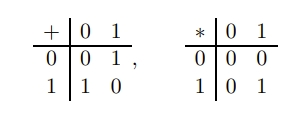
\includegraphics[width=0.3\textwidth]{figure/F_2_operator_table.png}
        \caption{}
    \end{figure}
    Since $\F_2=\{0,1\}$, it follows that a non-zero polynomial 
    in $\F_2[x]$ must be monic.
    The degree $3$ polynomials are of the form $x^3+ax^2+bx+c$,
    where each coefficient is $0$ or $1$, i.e. there are $2^3=8$ of them.\\
    If $c=0$, such a polynomial is reducible over $\F_2$ since it has $x$ as divisor.\\
    If $a=b=0,c=1$, assume $x^3+1=(x+a_0)(x^2+b_1x+b_0)=x^3+(b_1+a_0)x^2+(a_0b_1+b_0)x +a_0b_0$,
    then $a_0=b_0=b_1=1$ and so be reducible.\\
    If $a=b=c=1$, assume $x^3+x^2+x+1=(x+a_0)(x^2+b_1x+b_0)=x^3+(b_1+a_0)x^2+(a_0b_1+b_0)x +a_0b_0$,
    then $a_0=b_0=1$, $b_1=0$ and so be reducible.\\
    If $a=c=1$, $b=0$, assume $x^3+x^2+1=(x+a_0)(x^2+b_1x+b_0)=x^3+(b_1+a_0)x^2+(a_0b_1+b_0)x +a_0b_0$,
    then $a_0=b_0=1$, $b_1=0$ and so $a_0b_1+b_0=1\neq 0$. This is a contradiction and so be irreducible.\\
    If $b=c=1$, $a=0$, assume $x^3+x+1=(x+a_0)(x^2+b_1x+b_0)=x^3+(b_1+a_0)x^2+(a_0b_1+b_0)x +a_0b_0$,
    then $a_0=b_0=1$,$b_1=1$ and so $a_0b_1+b_0=0$. This is a contradiction and so be irreducible.\\
    Hence, $x^3+x^2+1$ and $x^3+x+1$ are irreducible.
\end{proof}

\begin{proposition}{}{}
    For $f \in F[x]$, 
    the quotient ring $F[x]/(f)$ is 
    a field if and only if 
    $f$ is irreducible over $F$.
\end{proposition}


% \begin{definition}{}{}
%     Let $F$ be a commutative ring with unity. 
%     $F$ is a field if $(F^*,\cdot)=(F\setminus\{0_F\},\cdot)$ is an abelian group.
% \end{definition}

% \begin{proposition}{}{}
%     Any finite subgroup of $F^*$ is cyclic.
% \end{proposition}

% \begin{proof}
%     proof referring to \href{https://proofwiki.org/wiki/Finite_Multiplicative_Subgroup_of_Field_is_Cyclic}{prook by proofwiki}
% \end{proof}


% \begin{proposition}{}{}
%     The only ideals of $F$ are $F$ and $(0)$.
% \end{proposition}

% \begin{proof}
%     proof referring to \ref{prop:field and ideals relation}
% \end{proof}

% \begin{proposition}{}{}
%     $F$ has no zero divisors.
% \end{proposition}
% \begin{proof}
    
% \end{proof}


\section{Reference}

\begin{itemize}
    \item \href{https://www.ma.imperial.ac.uk/~anskor/notesM2P4.pdf}{lecture note by anskor}
    \item \href{https://www.math.rwth-aachen.de/~Max.Neunhoeffer/Teaching/ff/ffchap1.pdf}{Introduction}
    \item \href{https://www.math.rwth-aachen.de/~Max.Neunhoeffer/Teaching/ff/ffchap2.pdf}{prime field}
\end{itemize}
\chapter{The Degree of Field Extension}\label{chp:6_2}

\section{Field extensions}


\begin{definition}{}{}
    Let $R$ be a ring with unity. A (Left) R-module is an additive abelian group $V$ together with a function mapping
    $R\times V\rightarrow V$(the image of $(a,x)$ being denoted $ax$) such that for all $a,b\in R$ and $x,y\in V$:\\
    (1) $1_Rx=x$\\
    (2) $(ab)x=a(bx)$\\
    (3) $(a+b)x=ax+bx$\\
    (4) $a(x+y)=ax+ay$ 
\end{definition}

\begin{remark}
    If $R$ is a field, then R-module is called a (left) vector space.
\end{remark}

\begin{definition}{}{}
    A field $L$ is an extension field of field $K$ if $K$ is a subfield of $L$. 
    And we denote the corresponding field extension by $L/K$.
\end{definition}

\begin{remark}
    with $R=K$ (the field of "scalars") and $V=L$ (the additive abelian group of "vectors"), we see that $L$ is a vector space over $K$.
    It then makes sense to speak of the dimension of $L$ over $K$.
\end{remark}


\begin{definition}{}{}
    Let $L/K$ be a field extension. The dimension of $L$ as a vector space over $L$
    is called the degree of the extension, written $[L:K]$.
    If $[L:K]<\infty$, we say that $L$ is a finite extension of $K$, or that the extension $L/K$ is finite.
\end{definition}

\begin{proposition}{}{}
    Let $L/M$ and $M/K$ be finite field extension, then
    \begin{align*}
        [L:K]=[L:M][M:K].
    \end{align*}
\end{proposition}

\begin{definition}{}{}
    For field $L$ and $\O\neq X\subset L$, the subfield (respectively, subring) generated by $X$
    is the intersection of all subfields (respectively, subrings) of $L$ that contain $X$.  
    i.e., the smallest subfield (resp. subring) of
    $F$ containing $X$.
\end{definition}

\begin{definition}{}{}
    Let $L/K$ be a field extension and $\O\neq X\subset L$. Then the subfield (respectively, subring)
    generated by $K\cup X$ is the subfield(respectively, subring) generated by $X$ over $K$ and is denoted $K(X)$ 
    (or, respectively, in the case of rings, $K[X]$).
    i.e., the smallest subfield (resp. subring) of $F$ containing $K\cup X$.
\end{definition}

\begin{definition}{}{}
    If $X=\{\alpha_1,\alpha_2,...,\alpha_n\}$, then the subfield $K(X)$ (respectively, subring $K[X]$)
    of $F$ is denoted $K(\alpha_1,\alpha_2,...,\alpha_n)$ (respectively, $K[\alpha_1,...,\alpha_n]$). 
    The field $K(\alpha_1,...,\alpha_n)$
    is a finitely generated extension of $K$. If $X=\{\alpha\}$ then $K(\alpha)$ is a simple extension of $K$.
\end{definition}

\begin{remark}
    The field $K(\alpha_1,...,\alpha_n)$ is a finitely generated extension of $K$ but it may not be a finite dimensional extension over $K$.
\end{remark}

\begin{theorem}{}{}
    Let $L/K$ be a field extension and $X\subseteq L$ and $\alpha$, $\alpha_i\in L$. Then\\
    (1) the subring $K[\alpha]$ consists of all elements of the form $f(\alpha)$ where $f$ is a polynomial with coefficients in $K$ (that is, $f\in K[x]$), i.e. 
    $K[\alpha]=\{f(\alpha):f(x)\in K[x]\}$. \\
    (2) the subring $K[\alpha_1, \alpha_2, . . . , \alpha_n]$ consists of all elements of the form $f(\alpha_1, \alpha_2, . . . , \alpha_n)$,
    where $f$ is a polynomial in $n$ indeterminates with coefficients in $K$ (that is,
    $f \in K[x_1, x_2, . . . , x_n]$); i.e. 
    $K[\alpha_1,...\alpha_n]=\{f(\alpha_1,...,\alpha_n):f(x_1,...,x_n)\in K[x_1,...,x_n]\}$. \\
    (3) $K(\alpha)=\{\frac{f(\alpha)}{g(\alpha)}:f(x),g(x)\in K[x] \text{ and } g(\alpha)\neq 0\}$. \\
    (4) $K(\alpha_1,...,\alpha_n)=\{\frac{f(\alpha_1,...,\alpha_n)}{g(\alpha_1,...,\alpha_n)}:f,g\in K[x_1,...,x_n]\text{ and } g(\alpha_1,...,\alpha_n)\neq 0\}$.
\end{theorem}

\begin{proof}
    (2) Let $S=\{f(\alpha_1,...,\alpha_n):f(x_1,...,x_n)\in K[x_1,...,x_n]\}$ and $X=\{\alpha_1,...,\alpha_n\}$. 
    Then $S\subset K[\alpha_1,...,\alpha_n]$,   
    as $K[\alpha_1,...,\alpha_n]$ is a subring of $L$ containing $K\cup X$ and $S$ is the collection of linear combination of elements of $K\cup X$.
    Conversely, if $f_1\in K[x_1,...,x_m]$ and $f_2\in K[x_1,...,x_n]$, as $f_1\pm f_2, f_1\cdot f_2 \in K[x_1,...,x_n]$, 
    then for $\alpha_1,...,\alpha_n$, 
    \begin{align*}
        f_1(\alpha_1,...\alpha_n) \pm f_2(\alpha_1,...\alpha_n) , f_1(\alpha_1,...\alpha_n) \cdot f_2(\alpha_1,...\alpha_n)\in S.
    \end{align*}
    Therefore, $S$ is an subring of $L$ and so a ring.
    Since $X\subset S$ ($\forall i$ , let $f(x_1,...,x_n)=x_i$ then $f(\alpha_1,...,\alpha_n)=\alpha_i$) and $K\subset S$ ($\forall k\in K$, Let $f(x_1,...,x_n)=k$ then $f(\alpha_1,...,\alpha_n)=k$)
    and $K[\alpha_1,...,\alpha_n]$ is the intersection of subring containing $K\cup X$, 
    $K[\alpha_1,...,\alpha_n]\subset S$. Hence, $K[\alpha_1,...,\alpha_n]=S$. 
\end{proof}


We now distinguish between two types of elements of an extension field.
This is fundamental to all that follows.

\begin{definition}{}{}
    Let $L/K$ be a field extension. 
    An element $\alpha\in L$ is algebraic over $K$ if $\alpha$ is a root of some nonzero polynomial $f\in K[x]$.
    If $\alpha$ is not a root of any nonzero $f\in K[x]$ then $\alpha$ is transcendental over $K$.
    $L$ is an algebraic extension of $K$ if every element of $L$ is algebraic over $K$.
    $L$ is a transcendental extension if at least one element of $L$ is transcendental over $K$.
\end{definition}


Let $L/K$ be a field extension and $\alpha\in L$ is algebraic over $K$.
We claim that $I=\{g(x)\in K[x]:g(\alpha)=0\}$ is a ideal in $K[x]$. 
In fact, for $f(x),g(x)\in I, h(x)\in K[x]$, $f(\alpha)\pm g(\alpha)=0$ and $h(\alpha)f(\alpha)=0$.
Since $K[x]$ is principal ideal domain, there exists unique monic polynomial $f(x)\in K[x]$
such that $I=(f(x))$. If $g(x)\in I=(f(x))$, then $f(x)|g(x)$. Hence, the degree of $f(x)$ is smallest in $I$. 
Now we prove $f(x)$ is irreducible in $K$. Suppose $f = gh$. 
Since $f(\alpha)=g(\alpha)h(\alpha)=0$ and $K$ is a field(hence also an integer domain), either $g(\alpha)=0$ or $h(\alpha)=0$. 
But this is a contradiction with the minimal degree on $f$, so $f$ must be irreducible.
such monic $f(x)$ is called the minimal polynomial of algebraic $\alpha$ over $K$.
The degree of $\alpha$ over $K$ is deg($f$).

\begin{example}{}{}
    The element $\sqrt[3]{3}\in\R$ is algebraic over $\Q$ since it is a root of $x^3-3\in\Q[x]$.
    Since $x^3-3$ is irreducible over $\Q$, it is the minimal polynomial of $\sqrt[3]{3}$ over $\Q$,
    and hence $\sqrt[3]{3}$ has degree $3$ over $\Q$.
\end{example}

\begin{example}{}{}
    Then element $i=\sqrt{-1}\in\C$ is algebraic over the subfield $\R$ of $\C$, since it is a root of the polynomial $x^2+1\in\R[x]$.
    Since $x^2+1$ is irreducible over $\R$, it is the minimal polynomial of $i$ over $\R$,
    and hence $i$ has degree $2$ over $\R$.
\end{example}

\begin{proposition}{}{}
    Every finite extension of $K$ is algebraic over $K$.
\end{proposition}
\begin{proof}
    Let $K$ be a finite extension of $K$ and let $[L:K]=m$.
    For $\alpha\in L$, then $m+1$ elements $1,\alpha,...,\alpha^m$ must be linearly dependent over $K$, i.e. must satisfy $a_0+a_1\alpha+\cdots +a_m\alpha^m=0$
    for some $a_i\in K$ (not all zero). Then $\alpha$ is algebraic over $K$.
\end{proof}


In the next two theorems, we classify simple extensions (first, extending by
a transcendental and second extending by an algebraic).


\begin{theorem}{}{transcendental extension basis}
    If $L/K$ is a field extension and $\alpha\in L$ is transcendental over $K$,
    then there is an isomorphism of fields $K(\alpha)\cong K(x)$ which is the identity when restricted to $K$, 
    where $K(\alpha)=\{\frac{f(\alpha)}{g(\alpha)}:f(x),g(x)\in K[x] \text{ and } g(\alpha)\neq 0\}$
    and $K(x)=\{\frac{f(x)}{g(x)}:f(x),g(x)\in K[x] \text{ and } g(x)\neq 0\}$
\end{theorem}

\begin{proof}
    Since $\alpha$ is transcendental then 
    $f(\alpha)\neq 0,g(\alpha)\neq 0$ for all nonzero $f,g\in K[x]$.
    Define $\varphi :K(x)\rightarrow L$ as $\frac{f}{g}\mapsto \frac{f(u)}{g(u)}$. 
    Since $\varphi(\frac{f_1}{g_1}+\frac{f_2}{g_2})=(\frac{f_1}{g_1}+\frac{f_2}{g_2})(u)=\frac{f_1}{g_1}(u)+\frac{f_2}{g_2}(u)=\varphi(\frac{f_1}{g_1})+\varphi(\frac{f_2}{g_2})$
    and $\varphi(\frac{f_1}{g_1}\cdot \frac{f_2}{g_2})=\frac{f_1}{g_1}\cdot \frac{f_2}{g_2}(u)= \frac{f_1}{g_1}(u)\cdot \frac{f_2}{g_2}(u)=\varphi(\frac{f_1}{g_1})\varphi(\frac{f_2}{g_2})$, 
    $\varphi$ is a homomorphism. Now for $\frac{f_1}{g_1}\neq \frac{f_2}{g_2}$, then $f_1g_2\neq f_2g_1$ and $f_1g_2-f_2g_1\neq 0$ (not the $0$ polynomial, that is). 
    Now $f_1(\alpha)g_2(\alpha)-f_2(\alpha)g_1(\alpha)\neq 0$ (or else $\alpha$ is algebraic over $K$), and so
    $\varphi(\frac{f_1}{g_1})=\frac{f_1(u)}{g_1(u)}\neq \frac{f_2(u)}{g_2(u)}=\varphi(\frac{f_2}{g_2})$. 
    Therefore, $\varphi$ is one to one. Also, $\varphi$ is the identity on $K$ (treating $K$ as a subfield of $K(x)$; think of $K$ as the constant rational functions in $L(x)$).
    So the image of $\varphi$ is $K(\alpha)$. So $\varphi$ is an isomorphism from $K(x)$ to $K(\alpha)$ which is the identity on $K$.
\end{proof}

\begin{remark}
    Theorem \ref{thm:transcendental extension basis} tells us what elements of the transcendental extension $K(\alpha)$ of $K$
    "look like":
    \begin{align*}
        \frac{f(\alpha)}{g(\alpha)}, \text{ where } f,g\in K[x] \text{ and } g(\alpha)\neq 0 
    \end{align*}
\end{remark}

\begin{theorem}{}{algebraic extension basis}
    If $L/K$ is a field extension and $\alpha\in L$ is algebraic over $K$, then\\
    (1) $K(\alpha)=K[\alpha]$;\\
    (2) $K(\alpha)\cong K[x]/f(x)$ where $f\in K[x]$ is the minimal polynomial of $\alpha$ with degree $n \geqs 1$ over $K$;\\
    (3) $[K(\alpha):K]=n$;\\
    (4) $\{1_K,\alpha,\alpha^2,...,\alpha^{n-1}\}$ is a basis of the vector space $K(\alpha)$ over $K$;\\
    (5) every element of $K(\alpha)$ can be written uniquely in the form $a_0+a_1\alpha+a_2\alpha^2+...+a_{n-1}\alpha^{n-1}$ where each $a_i\in K$.
\end{theorem}


\begin{proof}
    (1) and (2): 
    Define $\varphi: K[x]\rightarrow K[\alpha]$ as $g\mapsto g(\alpha)$. 
    Then clearly $\varphi$ is a ring homomorphism. By the form of elements of $K[x]$, $\varphi$ is onto. 
    Since $K$ is a field, $K[x]$ is a principal ideal domain.
    So $\Ker(\varphi)=(f)$ for some $f\in K[x]$ as $\Ker(\varphi)$ is an ideal. 
    Since $\alpha$ is algebraic and $\varphi(f)=f(\alpha)=0$, $\Ker(f)\neq \{0\}$.
\end{proof}



\begin{remark}
    Theorem \ref{thm:algebraic extension basis} tells us what elements of the algebraic extension $K(\alpha)$ of $K$
"look like". That is, there exists a fixed $n\in\N$ such that every element of $K(\alpha)$ is of the form $a_0+a_1\alpha+...+a_{n-1}\alpha^{n-1}$
for some $a_i\in K$.
\end{remark}

\begin{example}{}{}
    Consider the simple extension $\R(i)$ of $\R$. We saw earlier that $i$ has minimal polynomial $x^2+1$
    over $\R$. So $\R(i)\cong \R[x]/(x^2+1)$, and $\{1,i\}$ is a basis for $\R(i)$ over $\R$.
    So $\R(i)=\{a+bi:a,b\in\R\}=\C$.
\end{example}

\begin{example}{}{}
    Consider the simple extension $\Q(\sqrt[3]{3})$ of $\Q$. 
    We saw earlier that $\sqrt[3]{3}$ has minimal polynomial $x^3-3$ over $\Q$.
    So $\Q(\sqrt[3]{3})\cong \Q[x]/(x^3-3)$, and $\{1,\sqrt[3]{3},(\sqrt[3]{3})^2\}$ is a basis for $\Q(\sqrt[3]{3})$ over $\Q$.
    So $\Q(\sqrt[3]{3})=\{a+b\sqrt[3]{3}+c(\sqrt[3]{3})^2:a,b,c\in\Q\}$.
\end{example}

Note that we have been assuming that both $K$ and $\alpha$ are embedded in some larger field $F$. Next,
we will consider constructing a simple algebraic extension without reference to a previously given
larger field, i.e. “from the ground up”.
The next result, due to Kronecker, is one of the most fundamental results in the theory of fields:
it says that, given any non-constant polynomial over any field, there exists an extension field in
which the polynomial has a root.


\begin{theorem}{Kronecker's Theorem}{Kronecker's Theorem}
    If $K$ is a field and $f\in K[x]$ a monic irreducible polynomial of degree $n$, 
    then there exists a simple extension field $L=K(\alpha)$ of $K$ such that $\alpha\in L$ and $f$ is the minimal polynomial of $\alpha$. 
\end{theorem}



\begin{theorem}{}{}
    If $L$ is a finite dimensional extension field of $K$, then $L$ is 
    finitely generated and algebraic over $K$.
\end{theorem}


\begin{theorem}{}{}
    Let $L$ be an extension field of $K$. Then 
    $[L:K]<\infty$ iff there exists finite algebraic $\alpha_1,...,\alpha_n\in L$ over $K$
    such that $K(\alpha_1,...,\alpha_n)=L$.
\end{theorem}

\section{Splitting fields}

Given a polynomial, we now want an extension field which contains all its roots.

\begin{definition}{}{}
    Let $f\in K[x]$ be polynomial of positive degree and $F$ an extension field of $K$.
    Then we say that $f$ splits in $F$ if $f$ can be written as a product of linear factors in $F[x]$,
    i.e. if there exist elements $\alpha_1,\alpha_2,...,\alpha_n\in F$ such that
    \begin{align*}
        f=a(x-a_1)\cdots (x-\alpha_n)
    \end{align*}
    where $a$ is the leading coefficient of $f$.
    The field $F$ is called a splitting field of $f$ over $K$ if it splits in $F$ and $F=K(\alpha_1,...,\alpha_n)$. 
\end{definition}
\begin{remark}
    a splitting field $F$ of a polynomial $f$ over $K$ is an extension field containing all
    the roots of $f$, and is "smallest possible" in the sense that
    no subfield of $F$ contains all roots of $f$.
    The following
result answers the questions: can we always find a splitting field, and how many are there?
\end{remark}

\begin{theorem}{Existence and uniqueness of splitting field}{Existence and uniqueness of splitting field}
    (1) If $K$ is a field and $f$ any polynomial of positive degree in $K[x]$,
    then there exists a splitting field of $f$ over $K$.\\
    (2) Any two splitting fields of $f$ over $K$ are isomorphic under an isomorphism which keeps the elements of $K$ fixed and
    maps roots of $f$ into each other.
\end{theorem}

So, we may therefore talk of the splitting field of f over K. It is obtained by adjoining to $K$
finitely many elements algebraic over $K$, and so it is a finite extension.
of K.

\begin{example}{}{}
    Find the splitting field of the polynomial $f=x^2+2\in \Q[x]$ over $\Q$.
\end{example}

Up to now we have been saying 'a' splitting field. Theorem\ref{thm:Existence and uniqueness of splitting field} 
give us the right to speak of the splitting field of a given polynomial $f$
over a given field $K$. We write it as $\text{SF}_K ( f )$.

Splitting fields will be central to our characterization of finite fields, in the next chapter.

\section{Reference}
\begin{itemize}
    \item \href{https://faculty.etsu.edu/gardnerr/5410/notes/V-1.pdf}{Section V.1. Field Extensions}
    \item \href{https://mdu.ac.in/UpFiles/UpPdfFiles/2021/Jun/4_06-28-2021_11-45-05_Theory%20of%20Field%20Extensions_(20MAT22C1).pdf}{THEORY OF FIELD EXTENSIONS}
    \item \href{https://feog.github.io/chap3.pdf}{Field Theory}
    \item \href{https://mathstat.dal.ca/~yanghs/notes.php?name=Galois}{lecture notes by yanghs}
    \item \href{https://faculty.etsu.edu/gardnerr/5410/Beamer-Proofs/Proofs-V-1.pdf}{lecture notes by gardnerr}
    \item \href{https://www.math.rwth-aachen.de/~Max.Neunhoeffer/Teaching/ff/ffchap2.pdf}{Some field theory}
\end{itemize}
\chapter{Algebraic Extension}\label{chp:6_3}


\chapter{Finite Field}\label{chp:6_4}

We have seen, in the previous chapters, some examples of finite fields. For example, the quotient
ring $\Z/p\Z$ (when $p$ is a prime) forms a field with $p$ elements which may be identified with the
Galois field $\F_p$ of order $p$.

The fields $\F_p$ are important in field theory.
Since every finite field must have characteristic $p$, 
this helps us to classify finite fields.

\begin{lemma}{}{finite field cardinality lemma}
    Let $F$ be a finite field containing a subfield $K$ with $q$ elements. Then $F$ has $q^m$ elements,
    where $m=[F:K]$.
\end{lemma}
\begin{proof}
    $F$ is a vector space over $K$, finite-dimensional since $F$ is finite.
    Denote this dimension by $m$, then $F$ has a basis over $K$ consisting of $m$ elements,
    say $\alpha_1,...,\alpha_m$. Every element of $F$ can be uniquely represented in the form
    $k_1\alpha_1+...+k_m\alpha_m$ (where $k_1,...,k_m\in K$).
    Since each $k_i\in K$ can take $q$ values, $F$ must have exactly $q^m$ elements.
\end{proof}

We are now ready to answer the question: "What are the possible cardinalities for finite fields?"

\begin{proposition}{}{}
    Let $F$ be a finite field.
    Then $F$ has $p^n$ elements, where the prime $p$ is the characteristic of $F$ and 
    $n$ is the degree of $F$ over its prime subfield.
\end{proposition}
\begin{proof}
    Since $F$ is finite, it must have characteristic $p$ for some prime $p$ for some prime $p$.(by corollary\ref{cor:finite field prime characteristic})
    Thus, the prime subfield $K$ of $F$ is isomorphic to $\F_p$ (by proposition\ref{prop:prime subfield isomorphic to Q or Fp}), 
    and so contains $p$ elements. By lemma\ref{lem:finite field cardinality lemma}, $F$ has $p^n$ elements.
\end{proof}

So, all finite fields must have prime power order - 
there is no finite field with $6$ elements, for example.
We next ask: does there exist a finite field of order $p^n$
for every prime power $p^n$? How can such fields be constructed?
We can take the prime fields $\F_p$ and construct other finite
fields from them by adjoining roots of polynomials. If $f \in \F_p[x]$ is irreducible of degree $n$ 
over $\F_p$, by Kronecker's Theorem\ref{thm:Kronecker's Theorem}, 
then adjoining a root of $f$ to $\F_p$ yields a finite field of $p^n$
elements. However, it is not clear whether
we can find an irreducible polynomial in $\F_p[x]$ of degree $n$, 
for every integer $n$.

The following two lemmas will help us to characterize fields using root adjunction.


\section{Reference}

\begin{itemize}
    \item \href{https://www.math.rwth-aachen.de/~Max.Neunhoeffer/Teaching/ff/ffchap3.pdf}{Finite fields}
\end{itemize}
\chapter{Normal Extension and Separable Extension}\label{chp:6_5}

\section{Normality}

\begin{definition}{}{}
    An algebraic field extension $L/K$ is normal 
    if for all $\alpha\in L$,
    the minimal polynomial of $\alpha$ splits in $L$.
\end{definition}

\begin{lemma}{}{}
    Let $L/K$ be an algebraic extension. 
    Then $L/K$ is normal if and
    only if every irreducible polynomial over $K$ either has no roots in $L$ or splits in $L$.
\end{lemma}
\begin{proof}
    
\end{proof}

\begin{example}{}{}
    $\Q(\sqrt[3]{2})$
\end{example}

\begin{proposition}{}{}
    Let $L/K$ be a field extension. Then
    \begin{align*}
        L= \text{SF}_K ( f ) \text{ for some nonzero $f\in K[x]$}
        \Leftrightarrow L/k \text{ is finite and normal}.
    \end{align*}
\end{proposition}

\section{Normality}

\begin{definition}{}{}
    An irreducible polynomial over a field is separable if it has no
    repeated roots in its splitting field.
\end{definition}
\begin{remark}
    Formally, for a polynomial $f (x) \in K[x]$ 
    and a root $\alpha$ of $f$ in some extension $L$ of $K$, 
    we say that $\alpha$ is a repeated root if $(x - \alpha)^2| f (x)$ in $L[x]$.
\end{remark}
\begin{remark}
    Equivalently, an irreducible polynomial $f \in K[x]$ is separable 
    if it splits into distinct linear factors in $\text{SF}_K (f)$:
    \begin{align*}
        f(x)=a(x-\alpha_1)\cdots (x-\alpha_n)
    \end{align*}
    for some $a\in K$ and distinct $\alpha_1,...,\alpha_2\in \text{SF}_K(f)$.
    Put another way, an irreducible $f$ is separable if and if only it has deg$(f)$ distinct roots in its splitting field. 
\end{remark}

\begin{example}{}{}
    $x^3-2\in\Q[x]$ is separable, since it has $3$ distinct roots in $\C$,
    hence in its splitting field.
\end{example}



\section{Reference}

\begin{itemize}
    \item \href{https://www.maths.ed.ac.uk/~tl/gt/gt.pdf}{Normality; P98}
    \item \href{https://www.maths.ed.ac.uk/~tl/gt/gt.pdf}{Separability; P105}
\end{itemize}

\chapter{Exercise about Field}

\begin{exercise}{}{}
    Every finite integral domain with at least two elements is a field.
\end{exercise}

\begin{proof}
    Let $R$ be an finite integral domain with at least two elements. Then $R$ is commutative and satisfys cancellation law.
    Since $R\setminus\{0\}$ is finite and a multiplication semigroup, $R\{0\}$ is a group. Hence, $R$ is a field. 
\end{proof}

\begin{exercise}{}{}
    Let $L/M$ and $M/K$ be field extension. If $[L:K]$ is prime, then either $M=K$ or $M=L$.
\end{exercise}

\begin{proof}
    Since $[L:K]=[L:M][M:K]$ and $[L:K]$ is prime, either $[L:M]=1$ or $[M:K]=1$.
    If $[L:M]=1$, there exists a basis of $L$ over $M$ consisting of a single element. 
    In other words, there exists a $v\in L$ with the property that every element of $L$
    can be written as $mv$ for some $m\in M$. In particular, $1_M\in L$, so $1_M=m_0v$ 
    for some $m_0\in M$.
    Hence $v$ is the inverse of $m_0\in M$. Hence, $v\in M$. 
    Now every element of $L$ is a product of two elements of $M$, 
    hence every element of $L$ 
    is in $M$. Also, $M\subseteq L$ and so $M=L$. Similarly, if $[M:K]=1$, then $M=K$.
\end{proof}

\begin{exercise}{}{}
    Let $\alpha,\beta\in \Q(i)$, then $\alpha=\beta=0$ iff $\alpha^2+2\beta^2=0$.
\end{exercise}

\begin{proof}
    $\Q(i)=\{a+bi:a,b\in \Q\}$, so $\text{dim}_{\Q}(\Q(i))= 2$ and $\{1,i\}$ is a basis of $\Q(i)$. 
    Suppose $\alpha=a_1+b_1i$, $\beta=a_2+b_2i$\\
    ($\Rightarrow$): $\alpha=\beta=0$, then $\alpha^2+2\beta^2=0^2+2\cdot 0^2=0$.\\
    % ($\Leftarrow$): The coordinates of $\alpha^2+2\beta^2$ under $\{1,i\}$ is ($a_1^2+2a_2^2$, $b_1^2+2b_2^2$). 
    % If $\alpha^2+2\beta^2=0$, then $a_1^2+2a_2^2=0$ and $b_1^2+2b_2^2=0$. So $a_1=a_2=b_1=b_2=0$ and then $\alpha=\beta=0$.
    ($\Leftarrow$): Suppose neither $\alpha$ or $\beta$ equal $0$, then $\sqrt{2}i=\sqrt{-2}=\frac{\alpha}{\beta}\in \Q(i)$. 
    This is a contradiction as the coefficients of element in $\Q(i)$ under $\{1,i\}$ must be rational. 
    Hence, $\alpha=\beta=0$. 
\end{proof}

\begin{exercise}{}{}
    Let $L/K$ be field extension.
    For $\alpha,\beta\in L$ algebraic over $K$ with the same minimal polynomial then $K(\alpha)\cong K(\beta)$.
\end{exercise}

\begin{proof}
    Suppose $f$ is the minimal polynomial of $\alpha,\beta\in L$ over $K$, then $K(\alpha)\cong K[x]/f(x)$ and $K(\beta)\cong K[x]/f(x)$.
    Then there exist isomorphisms $\varphi: K(\alpha)\rightarrow K[x]/f(x)$ and $\mu: K(\beta)\rightarrow K[x]/f(x)$. 
    Then $\psi=\mu^{-1}\varphi:K(\alpha)\rightarrow K(\beta)$ is a isomorphism and so $K(\alpha)\cong K(\beta)$.
\end{proof}



\begin{exercise}{}{}
    Let $L/K$ be field extension. For $\alpha\in L$ with a minimal polynomial of odd degree in $K$ then $K(\alpha)=K(\alpha^2)$
\end{exercise}


\begin{proof}
    For $s\in K(\alpha^2)$, there exist $f,g\in K[x]$ such that $g(\alpha^2)\neq 0$ and 
    $s=\frac{f(\alpha^2)}{g(\alpha^2)}=\frac{a_0+a_1\alpha^2+...+a_n(\alpha^2)^n}{b_0+b_1\alpha^2+...+b_m(\alpha^2)^m}$
    $=\frac{a_0+a_1\alpha^2+...+a_n(\alpha)^{2n}}{b_0+b_1\alpha^2+...+b_m(\alpha)^{2m}}=\frac{f_1(\alpha)}{g_1(\alpha)}\in K(\alpha)$. 
    Hence, $K(\alpha^2)\subseteq K(\alpha)$. 
    Now for $f(x)=x^2-\alpha^2\in K(\alpha^2)[x]$, $f(\alpha)=0$. 
    Thus, $[K(\alpha):K(\alpha^2)]=1$ or $2$.
    If $[K(\alpha):K(\alpha^2)]=2$, $[K(\alpha):K]=[K(\alpha):K(\alpha^2)][K(\alpha^2):K]=2[K(\alpha^2):K]$.
    This is a contradiction as $[K(\alpha):K]$ is odd.
    Hence, $[K(\alpha):K(\alpha^2)]=1$ and so $K(\alpha)=K(\alpha^2)$.
\end{proof}


\begin{exercise}{}{}
    Let $K$ be a subfield of $\C$. If $a,b\in K$ and $\sqrt{a},\sqrt{b},\sqrt{ab}$ is not in $K$,
    then $[K(\sqrt{a},\sqrt{b}):K]=4$.
\end{exercise}

\begin{proof}
    Firstly, we claim that $K(\sqrt{a},\sqrt{b})=K(\sqrt{a})(\sqrt{b})$. In fact, 
    for $s\in K(\sqrt{a},\sqrt{b})$, 
    there exists $f,g\in K[x_1,x_2]$ and $f_1,g_1\in K(\sqrt{a})[x]$ such that $g(\sqrt{a},\sqrt{b})\neq 0$, $g_1(\sqrt{b})\neq 0$ 
    and $s=\frac{f(\sqrt{a},\sqrt{b})}{g(\sqrt{a},\sqrt{b})}=\frac{f_1(\sqrt{b})}{g_2(\sqrt{b})}$.
    Hence, $K(\sqrt{a},\sqrt{b})\subseteq K(\sqrt{a})(\sqrt{b})$.
    Similarly, $K(\sqrt{a},\sqrt{b})\supseteq K(\sqrt{a})(\sqrt{b})$ and so equality holds.
    Then, $[K(\sqrt{a},\sqrt{b}):K]=[K(\sqrt{a})(\sqrt{b}):K]=[K(\sqrt{a})(\sqrt{b}):K(\sqrt{a})][K(\sqrt{a}):K]=[L(\sqrt{b}):L][L:K]$, where $L=K(\sqrt{a})$.
    By $\sqrt{a}\notin K$, $[L:K]=2$. So it suffices to show that $[L(\sqrt{b}):L]=2$. It holds only if $\sqrt{b}\notin L$.
    Suppose $\sqrt{b}\in L$, then $\sqrt{b}=r+s\sqrt{a},r,s\in K$. But that is impossible since squaring yields 
    $a=r^2+bs^2+2rs\sqrt{b}$, which contradicts hypotheses as follows:\\
    if $rs\neq 0$, then $\sqrt{b}=\frac{a-r^2-bs^2}{2rs}\in K$ as $a,b,r,s\in K$;\\
    if $s=0$, then $a=r^2$ and $\sqrt{a}=r\in K$;\\
    if $r=0$, then $a= bs^2\Rightarrow \sqrt{ab}=bs\in K$.\\
    Hence, $\sqrt{b}\notin L$ and so $[L(\sqrt{b}):L]=2$.
    Then, $[K(\sqrt{a},\sqrt{b}):K]=4$.
\end{proof}

\begin{exercise}{}{}
    Let $\Q$ be rational field and $p\in\Z$ is prime. Then $\Q(\sqrt{p},\sqrt[3]{p},\sqrt[4]{p,\sqrt[5]{p}},...)$ is a infinte algebraic extension of $\Q$.
\end{exercise}

\begin{exercise}{}{}
    Let $\F_2=\{0,1\}$ is a finite field of two elements. Find out all the irreducible polynomial with two degree and three degree in $\F_2$.
\end{exercise}

\begin{exercise}{}{}
    Let $p\in\Z$ is prime and $\F_p$ is a finite field with $p$ elements. Then $\forall n\in \N$ and $n\geqs 1$, 
    $\F_{p^n}$ is the normal extension of $\F_p$
\end{exercise}




\section{Reference}
\begin{itemize}
    \item \href{https://math.stackexchange.com/questions/4314565/same-minimal-polynomial-gives-isomorphism}{Same minimal polynomial gives isomorphism}
    \item \href{https://math.stackexchange.com/questions/762460/minimal-polynomial-of-odd-degree}{Minimal polynomial of odd degree}
    \item \href{https://math.stackexchange.com/questions/113689/proving-that-left-mathbb-q-sqrt-p-1-dots-sqrt-p-n-mathbb-q-right-2n-f}{answer from mathexchage}
    \item \href{https://math.stackexchange.com/questions/925793/infinite-algebraic-extension-of-mathbbq}{Infinite algebraic extension of Q}
    \item \href{https://www.youtube.com/watch?v=sc9grztQClc}{Irreducible Polynomials in GF(2) of degree 1, 2 and 3.}
    \item \href{https://sites.math.washington.edu//~julia/teaching/505_Winter2010/notes.pdf}{$\F_{p^n}$ is the splitting field of $x^{p^n}-x$}.
\end{itemize}


\end{spacing}
\end{document}